\documentclass{book}
%trying to fit more on the page
\usepackage{geometry}
\geometry{a4paper, textwidth=17cm, textheight=23cm}

\usepackage{natbib}
\usepackage{listings}
\usepackage{verbatim}
\usepackage{array}
\usepackage{amsmath, amsthm}
\usepackage{graphviz}
\usepackage{graphicx}
\usepackage{makeidx}
\usepackage{glossaries}
\usepackage{hyperref} %take this out if you don't need links.

\hypersetup{
    colorlinks,%
    citecolor=black,%
    filecolor=black,%
    linkcolor=red,%
    urlcolor=blue
}

\usepackage{url}
\usepackage{float}
\usepackage{fancybox}
\newcommand{\HRule}{\rule{\linewidth}{0.5mm}}
%use of the float package allows for \begin{table}[H] which will not allow text to be placed before the image.
%\usepackage[english]{babel} % Quotes won't work without babel
%\usepackage[utf8]{inputenc}  % This is very important!
%usepackage[T1]{fontenc} % shite font
%\usepackage{tabularx}
\usepackage{multirow}
%\usepackage{pdflscape}
%\usepackage{rotating}

%\input{glossaryentries}
%\makeglossaries
%test because text is emerging before graphics in some instances.
%\raggedbottom
%\includeonly{chap1, appen1}
\begin{document}
%\title{Undergraduate Handbook}
%\author{The University of Sheffield \\ Department of Music\\}
%\date{\today}
%\maketitle

\frontmatter

\begin{titlepage}

\begin{center}


% Upper part of the page


\includegraphics[scale=0.2]{tuoslogo_cmyk_hi} \\


%\textsc{\LARGE Department of Music.}\\[1.5cm]


% Title
\HRule \\[0.4cm]
{ \huge \bfseries MUS119}\\[0.4cm]

\HRule \\[1.5cm]

% Author and supervisor
\begin{minipage}{0.6\textwidth}
\begin{flushleft} \large
Introduction to Studio\\
\end{flushleft}
\end{minipage}

\vfill

% Bottom of the page
{\large \today}

\end{center}

\end{titlepage}

\tableofcontents

\mainmatter
\graphicspath{{images//}}
\chapter{Dates and Times in history}
\label{datesnfolk}

\section*{A short list of dates, times and places that are of importance.}

%\begin{description}
%  \item[First] The first item
%  \item[Second] The second item
%  \item[Third] The third etc \ldots
%\end{description}


\begin{description}
\item [Charlemagne] In lands ruled by the Popes and the Franks, Charles - later to be called Chalemagne - had control over a vast kingdom taking in most of what is now France, Germany and Italy on/around 775. Chalemagne encouraged the pursuit of learning and people prospered. War was never far away however with the Vikings and the Magyars attacking in the late 10th Century. 
\item [Habsburg] Under Empirial rule, more local government was taken care of by hugely powerful families - dynasties, the largest of which was the Habsburgs. The first Habsburg `Emperor of Rome' was Rudolf IV 1272/1273. The Habsburg empire survived until 1806 when the title was abolished. 
\item [1066] The Normans, led by William landed on English soil on September 28, 1066 and ultimately defeated the king, Harold in the battle of Hastings. Because of familial alliances (or more probably their breakdown), William challenged Harold's claim to the throne. 
\item [The power of the church] The Crusades began in 1095 and started two centuries of violence between Christians and Muslims. 
\item [Law and Order] 1215 and King John signed Magna Carta, promising to abide by its laws. 
\item [The Black Death] Rather like Bird flu, the plague started somewhere far, far away but eventually reached every corner of the land. It reached London in 1349. With people tired and weak after war, it is hardly surprising they were susceptible. 
\item [The Hundred Years' War] Anglo-French relations were relatively stable due to the marital ties of Henry Plantagenet and Eleanor of Aquitaine. However, this was to break down when Edward III went to war against France in the defence of Aquitaine in 1357. 
\item [The Renaissance] The fifteenth and sixteenth centuries. Leonardo de Vinci (1452-1519), Michelangelo (1475-1564) Raphael (1483-1520). Who were the composers of the time? 
\item ...
\item ...
\item [Brave new world] Christopher Columbus sets sail in 1492. 
\item [Reformation] Martin Luther posts his 95 propositions in 1517 and the Protestant Catholic revolution had begun. 
\item [Elizabeth I] England and Spain had been allies through marriage but when Elizabeth succeeded the throne from Queen Mary (Catholic) in 1558, a division appeared. With Spain and Portugal now in league, war was to follow. Francis Drake was one of the heros of the war. 
\item [Shakespeare] With a gift for capturing the essence of the age Shakespeare (1564-1616) was an acclaimed writer in his time.
\item [The Thirty Years' War] Bitter rivalries between the Holy Roman Empire (dominated by the Habsburgs) and surrounding nations, notably France. Catholic fought Catholic (France vs. Roman Empire using Spanish armies). 
\item [Roundheads and Cavaliers] Death of Charles I in 1649. English civil war middle of the 17th Century. 
\item [The Sun King] Louis XIV as a puppet of the Church, attempts absolute rule. Future kings Louis XV and XVI gradually see their empire tumble into revolution. 
\item [The British in India] The British East India Company - something that just got out of hand. Read about the `black hole of Calcutta' (1756).
\item [Don't forget the East] Frederick the Great ruled over Prussia for over 40 years. 
\item [Canada] Britain vs. France batte for Canada in 1759
\item [Australia] Discovered by Cook in 1770 though seen by many before that time. 
\item [US Independence] Benjamin Franklin, Thomas Jefferson and John Adams in 1776
\item [Revolution] The storming of the Bastille in 1789. The rise, and ultimately the fall (1794) of `citizen Robespierre'. 
\item [Napoleon] leads his overstretched army in to Russia and to a wintry death in 1812.
\item [Communism] Karl Marx (1818-1883)
\item [Americans in Japan] After 1853, American ships sail into Yokohama and Nagasaki to trade with Japan. 
\item [Civil War in America] Abraham Lincoln (1809-1865) proclamation in 1862 to end slavery. 
\item [Russian Revolution] 1905 Tsar Nicholas II quashed a large uprising - Bloody Sunday. 
\item [First World War] Following the assassination of Archduke Franz Ferdinand by Serbian `Black Hand', Austria using Germany as ally decided to neutralise Serbia. Russia came to Serbia's defence. Although France was neutral they could not avoid being caught up in the war as Germany declared war on Russian and invaded Luxembourg prior to invading Belgium. Germany declared war on France. Britain came to Belguim's aid when the German's invaded. 1914, Britain and France were at war with Germany. 
\item [Battles] of Britain and WWII. 
\item [Other continuing battles with a history] Israelies and Palestinians. Key moments include independence of Israel in 1948. Pursuant to this and the division of Palestine, a continuance of Arab-Israeli conflicts that continue to this day.    
\end{description}





\chapter{The Romantic Symphony}
\label{romanticsymphony}

%\section{Scores}

\section{Brahms Symphony No 1 }
\begin{itemize}
\item Listen: \url{https://www.youtube.com/watch?v=o3a4v1TWUNo}
\item Score: \url{http://imslp.org/wiki/Symphony_No.1,_Op.68_%28Brahms,_Johannes%29}
\item Reading: \url{http://www.jstor.org/stable/pdfplus/20696500.pdf}
\end{itemize}

Symphony No.1 in C minor Op.68. Completed in 1876 but started in 1855 so interesting to probe the gestation period. 

Johannes Brahms (1833-1897, born in Hamburg). An exceptional body of work including works for piano, chamber ensemble, works for the female voice and four symphonies. Brahms was an excellent pianist and loved to be in love. His muse was the Clara Schumann. Brahms knew the Schumanns through their mutual friend and violin virtuoso Joseph Joachim. Unfortunately Robert Schumann was nearing the end of his life. He tried to commit suicide in 1854 and died in an asylum in 1856. Tragically sad end to the romantic composer's life. Brahms was superb at Lieder form but equally competent at the string quartet. With larger scale works, the violin concerto remains one of the key romantic concertos. 

\section{Europe in the middle 19th Century}
Europe was naturally going through political turmoil during the middle of the century. There were revolutions in France, Italy, Hungary and Germany. Technology was moving apace. Although the first known photograph was taken in 1827, it was not until the later part of the century that George Eastman created a method that was cheap enough to be mass-marketed (Kodak). Meanwhile Michael Faraday was making the first experiments generating electricity by passing magnets through coils of wire. By the end of the century street lighting was electric and the light bulb had been developed. 

Prior to Brahms' birth notable artistic endeavours included:
\begin{itemize}
\item Jane Austin: \textit{Pride and Prejudice} (1813)
\item Mary Shelly: \textit{\href{http://www.gutenberg.org/files/84/84-h/84-h.htm}{Frankenstein}} (1818)
\item Carl Maria von Weber: Der Freisch\"utz (1821)
\item John Constable: \textit{\href{http://www.nationalgallery.org.uk/paintings/john-constable-the-hay-wain}{The Hay Wain}} (1821)  
\end{itemize}

Der Freisch\"utz is perhaps best known because of the `Wolf's Glen' scene where magic bullets are cast and the devil is conjured. It is here that romantic ideas of the supernatural appear on stage and in music. In this respect the Hay Wain is both classical and romantic. The way nature was brought to life and the degree of subjective interpretation began to move painting from the figurative to the subjective. Alongside Constable we have the landscape painting of Joseph Turner (1775-1851). You can see the great attention to detail and figure but at the same time, an approach to colour that is bordering on the impressionist. 

Edgar Allen Poe introduced ideas of the supernatural and the macabre in his key texts of the mid 19th Century including `The Fall of the House of Usher', `The Pit and the Pendulum', and poems such as `\href{https://www.youtube.com/watch?v=0K6-wO94-6I}{The Raven}'.  

Going back further still, the American declaration of independence of 1776 (read about the Boston Tea Party) led others to believe in emancipation from dictators. In particular the French, who revolted against Louis XVI and Marie Antoinette in 1789 by storming the Bastille. 

And in 1812 Napoleon invaded Russia but this was the beginning of the end for him. The gruesome nature of war is captured in paintings such as Goya's `The Third of May 1808', during the Peninsular war between France and Spain. We see the French slaughtering helpless Spanish civilians.   

And of course in 1824 we have Beethoven's Choral Symphony, stretching musical form and forces to the maximum. 

The turmoil the romantic painting (see Turner's Snow Storm: Steam-Boat off a Harbour's Mouth of 1842) can be heard in music of Wagner in the middle of the century (Operas depicting salvation through death - Der fleiglende Holl\"ander, Tristan und Isolde for example) and in the writing of the Bront\"e sisters (Emily Bront\"e's \href{http://www.wuthering-heights.co.uk/index.php}{Wuthering Heights} of 1847 (\href{http://www.gutenberg.org/ebooks/768}{read it here}).

Verdi (1813-1901) was using his operas to investigate character - in particular their flaws and failings, famously drawing upon Shakespeare (for Macbeth(1865), and towards the end of the century, Otello(1887) and Falstaff(1893)). 
At the time Brahms was starting to write the First Symphony, Verdi had achieved fame with three operas: Rigoletto(1851), Il Trovatore(1853) and La Traviata(1853). But although Verdi might sound like Wagner, he did not know the man's music. Rigoletto is particularly tragic but endears itself through highly memorable arias such as `La donne \'e mobile'. Following hot on the heels of Verdi was Giacomo Puccini (1858-1924). Puccini heard a performance of Verdi's \textit{A\"ida} and this convinced him that the family business of organist was not for him. Puccini's first opera \textit{Manon Lescaut} (1893) was extremely successful and he is known as an opera composer. We will look at \textit{La Boh\`eme} (1896) - another masterpiece. 

Wagner's Ring cycle had come to completion and the Festspielhaus was to premiere \textit{Das Rheingold} on 13th August 1876. Brahms' First Symphony premiered on November 4, 1786. 

\section{Brahms Symphony No. 1: details} 

\subsection{First movement}

The movement begins with a slow introduction that highlights some of the key cells of the piece and focuses attention upon the strings and oboe, important declamatory instruments for the first movement. The opening introduction is marked \textit{Un poco sostenuto} and \textit{pesante} but this is interpreted wildly from conductor to conductor (A very brief search shows Andrew Manze's recording taking a brisk 2:16 with Mariss Jansons taking a ponderous 2:55 - and 40 seconds makes all the difference here) the movement picks up the pace for a spirited allegro. The strings present the theme in C minor.

\begin{figure}[H]
\centering
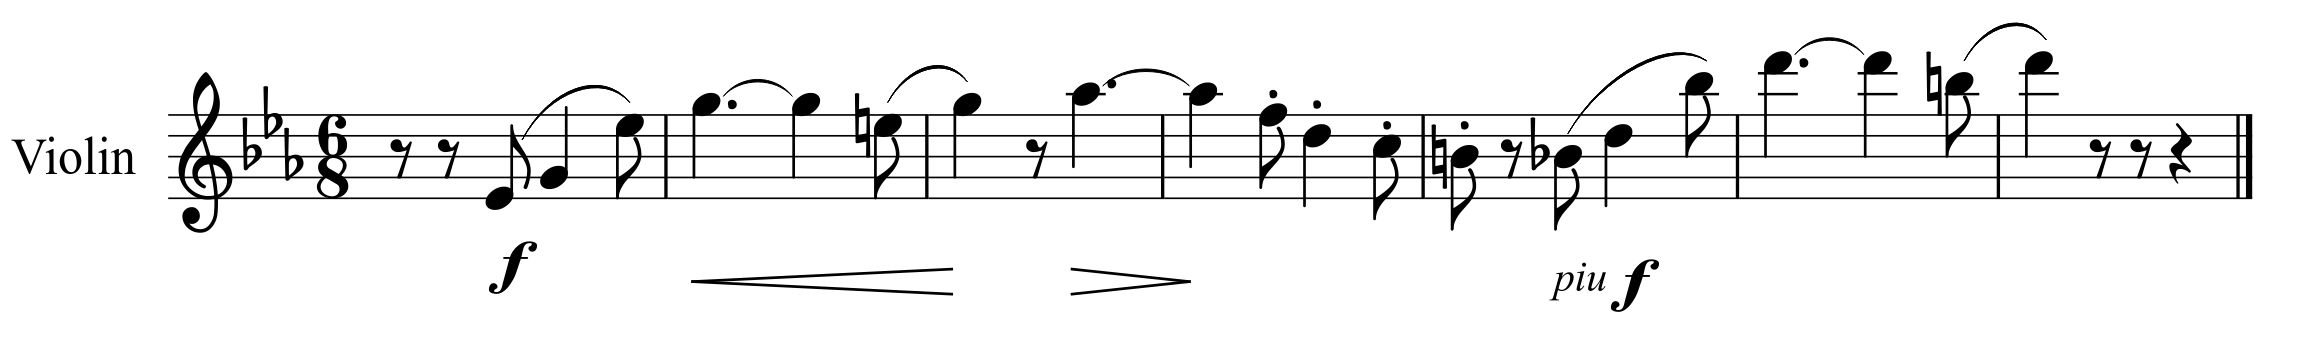
\includegraphics[scale=0.2]{brahms1mvt1a}\caption{Brahms Symphony No.1 mvt1 First subject}
\label{fig:b1m1first}
\end{figure}

At figure C a transition begins with lilting rhythms (important for driving the music forward during the development section). The movement slows and the oboe states the second theme.

\begin{figure}[H]
\centering
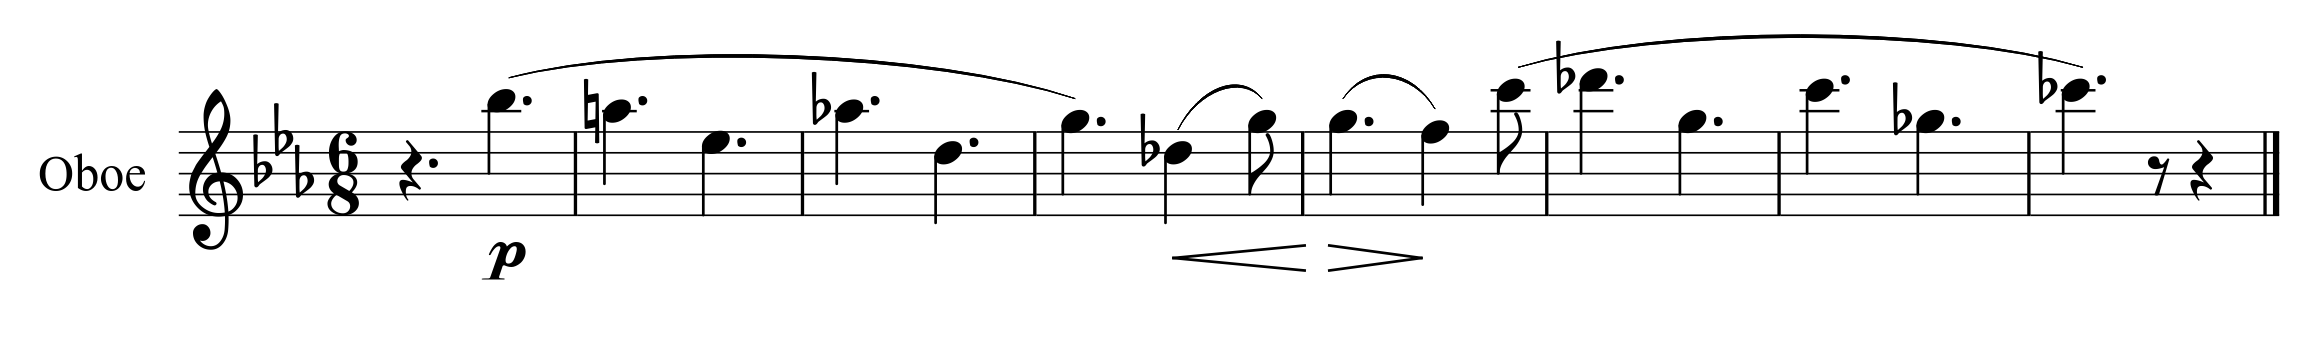
\includegraphics[scale=0.2]{brahms1mvt1b}\caption{Brahms Symphony No.1 mvt1 Second subject}
\label{fig:b1m1second}
\end{figure}

But it is not long before the pace picks up again with heavily articulated strings.

\begin{figure}[H]
\centering
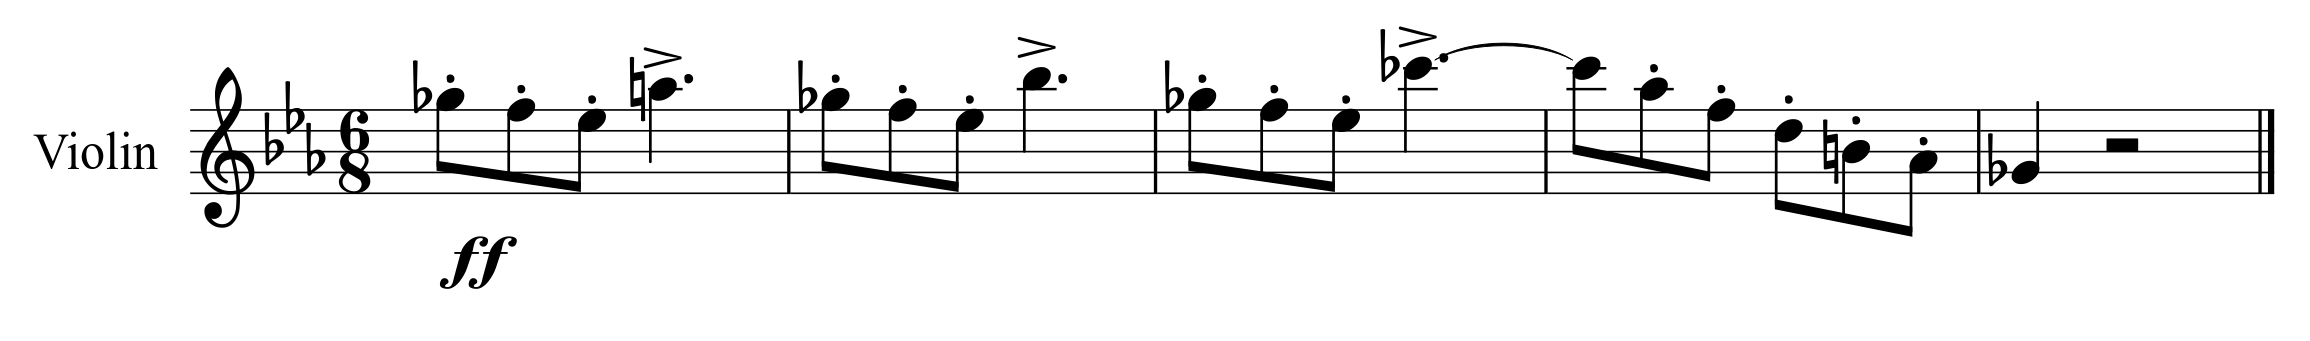
\includegraphics[scale=0.2]{brahms1mvt1c}\caption{Brahms Symphony No.1 mvt1 articulation 1}
\label{fig:b1m1rhythmic1}
\end{figure}

The exposition is not normally repeated (although Manze's recording does repeat). The move to B major is astonishing. 

Brahms makes a clever move as he develops the articulated theme from figure~\ref{fig:b1m1rhythmic1} towards something that mixes articulated and sustained (figure~\ref{fig:b1m1rhythmic2}).

\begin{figure}[H]
\centering
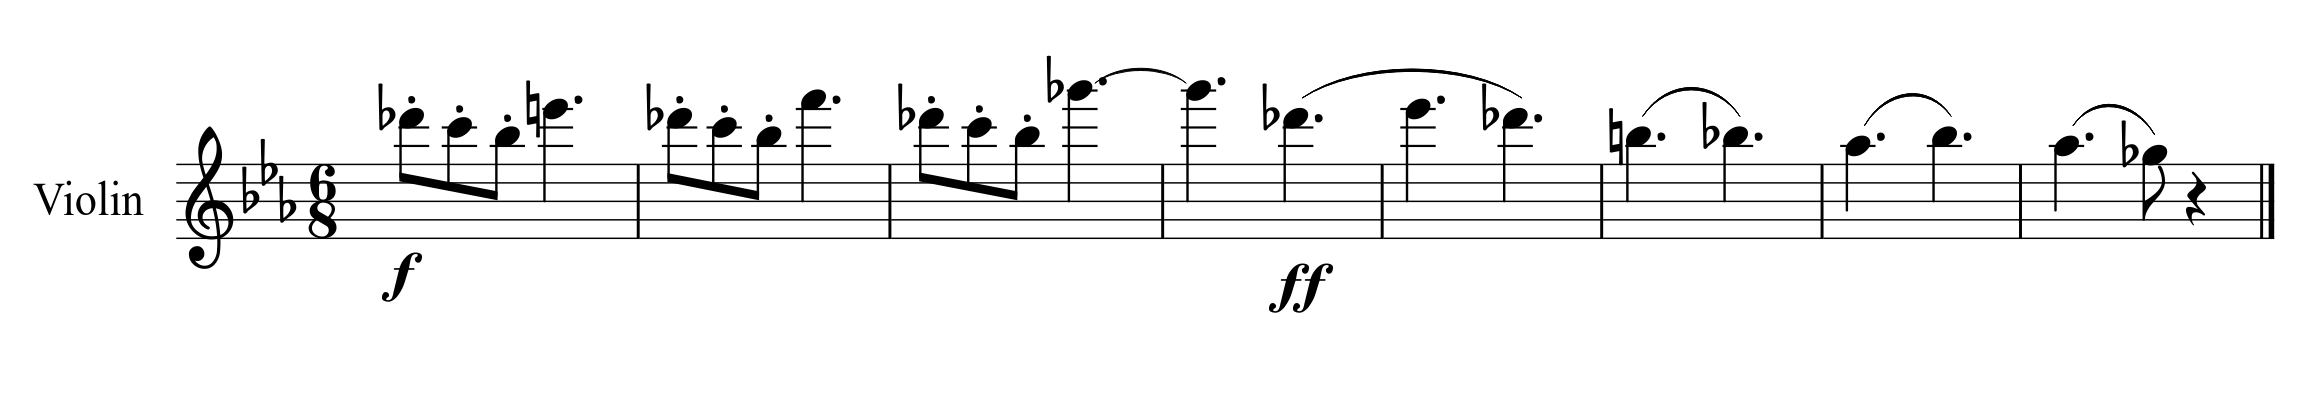
\includegraphics[scale=0.2]{brahms1mvt1d}\caption{Brahms Symphony No.1 mvt1 articulation 2}
\label{fig:b1m1rhythmic2}
\end{figure}

A huge sequential passage (bar 321) heralds the recapitulation in the home key and a major second subject return. 

After a heavily punctuated section alternating wind and strings, the coda seals the movement calmly but beguilingly contrasting major and minor modes leaving perhaps a sense of unease at the end.  

\subsection{Second movement} 
The second movement is an altogether stately affair. The oboe and strings again share the key themes but there is less thematic unity than in the previous movement. The slow solo violin heralds the end of the movement. 

There are some very interesting chromatic passages at the close of this movement that suddenly remind us of the opening of the symphony. 

\begin{figure}[H]
\centering
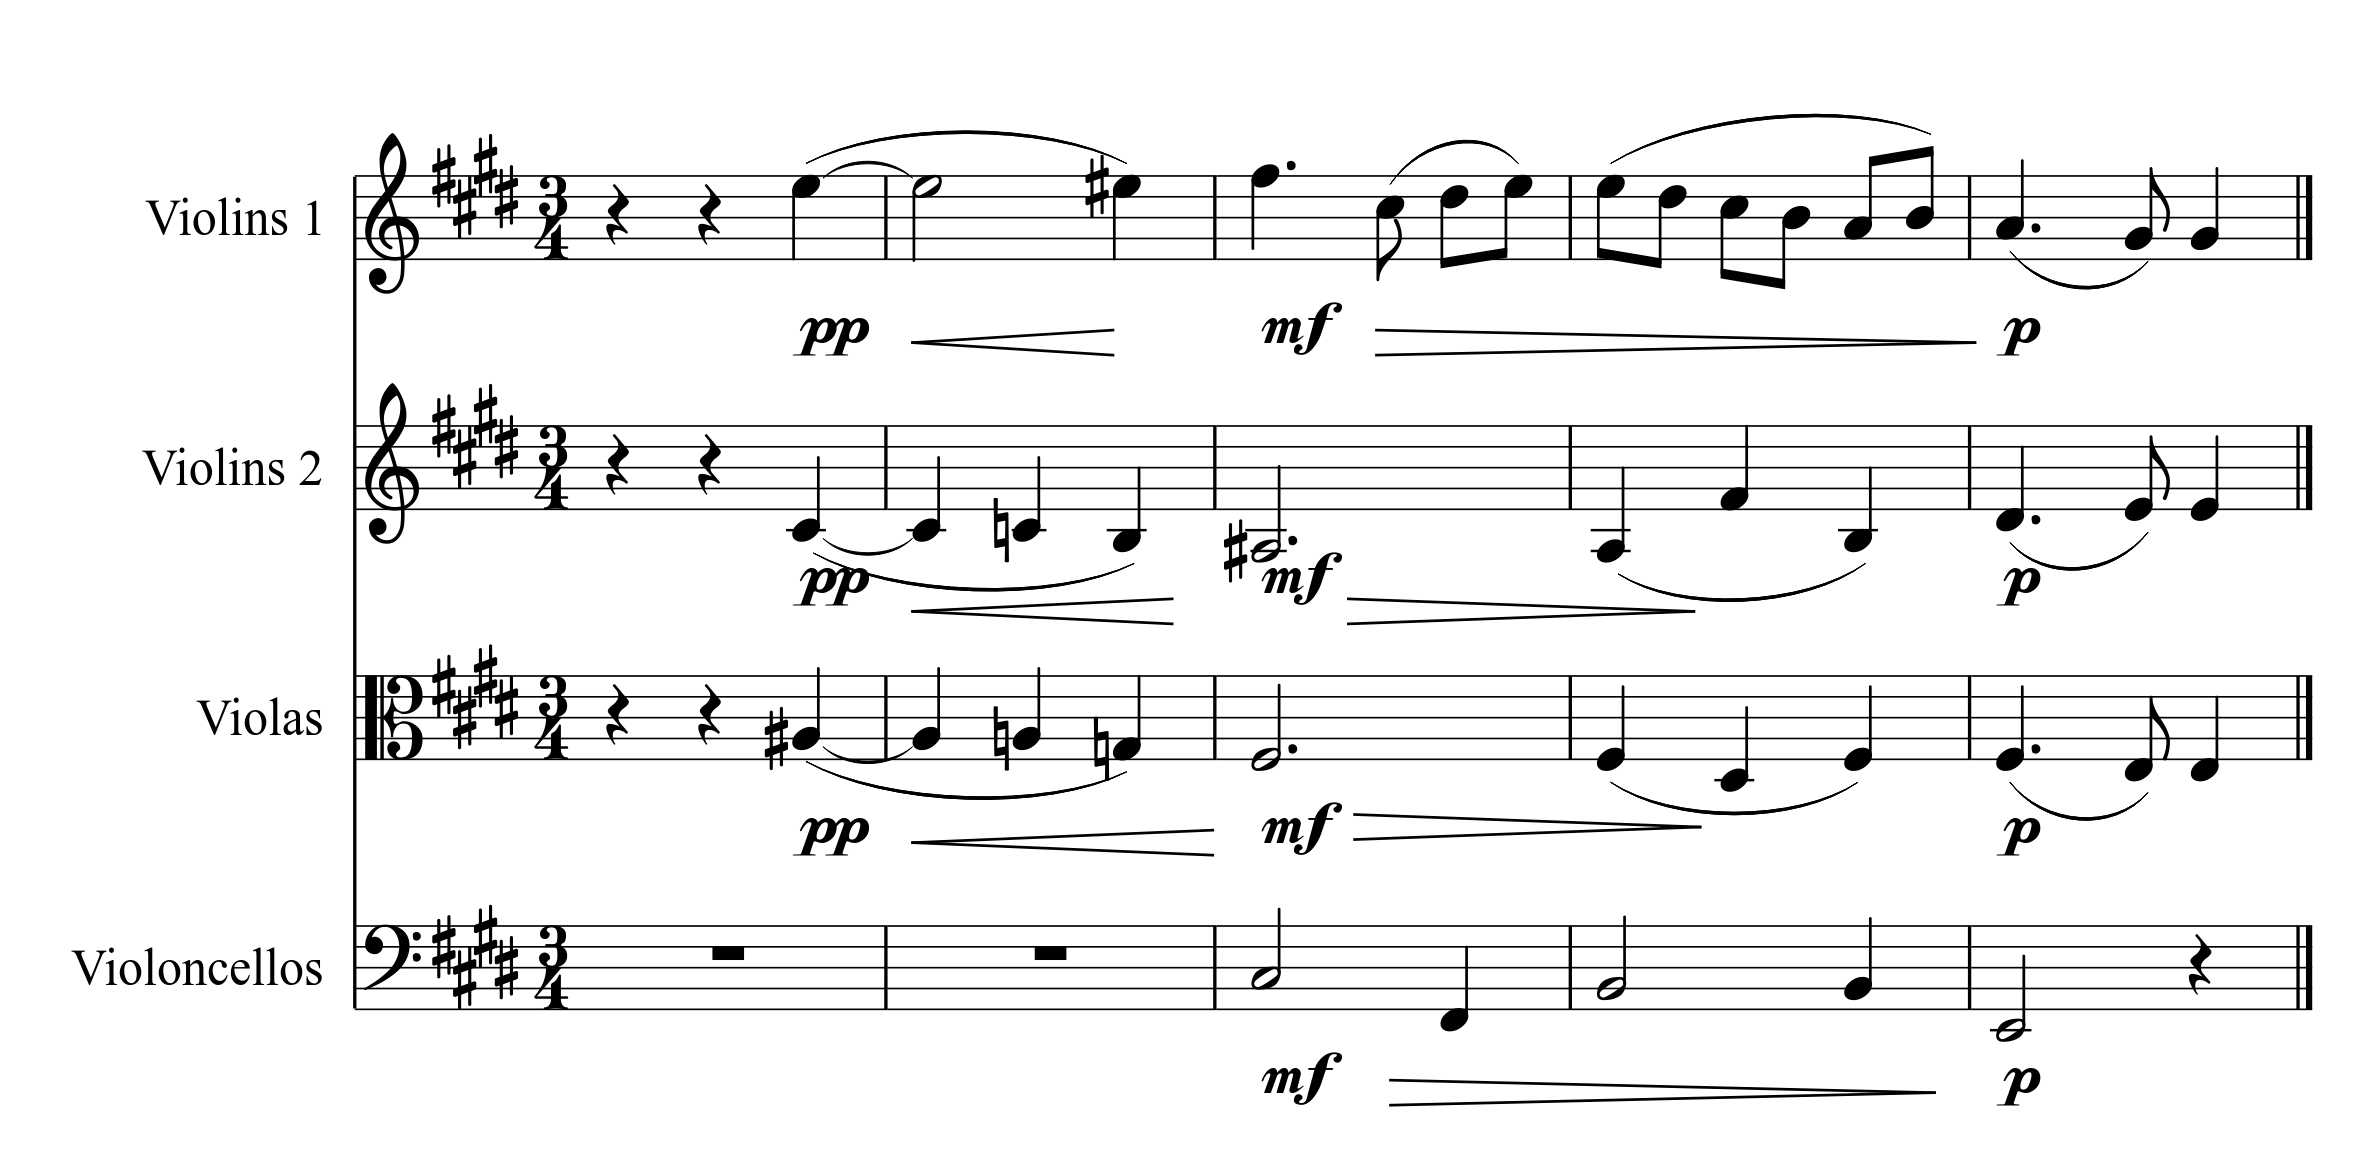
\includegraphics[scale=0.2]{brahms1mvt2chromatic}\caption{Brahms Symphony No.1 mvt2 bar 116}
\label{fig:b1m2chromatic}
\end{figure}

with...

\begin{figure}[H]
\centering
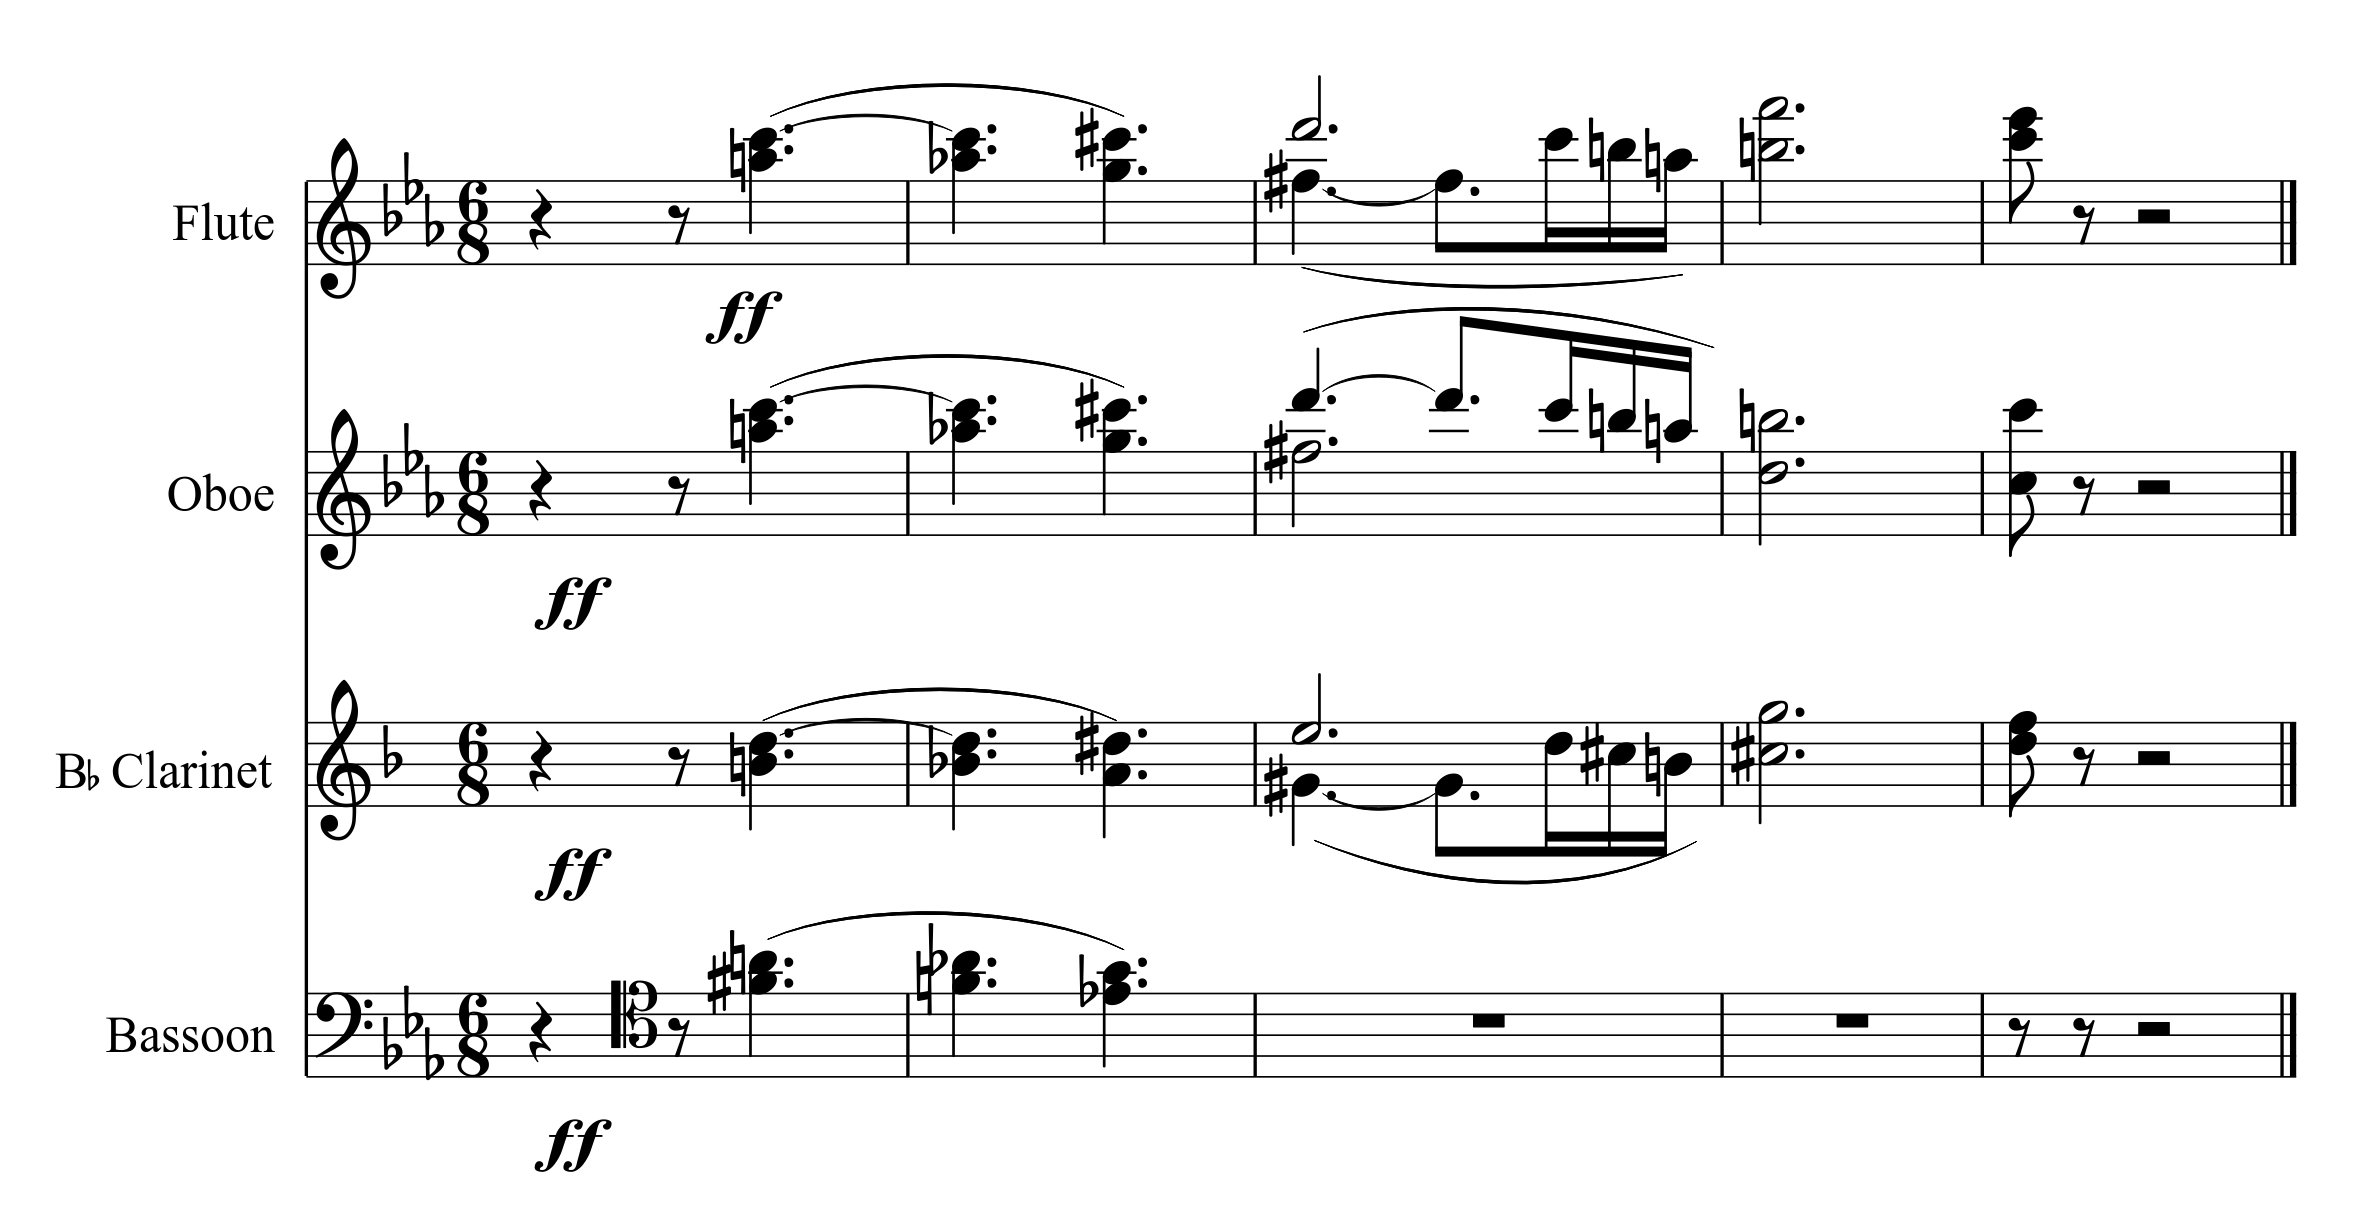
\includegraphics[scale=0.2]{brahms1mvt1chromatic}\caption{Brahms Symphony No.1 mvt1 Allegro woowind bar 38}
\label{fig:b1m2chromatic}
\end{figure}

\subsection{Third movement}
The third movement is therefore much lighter in design and is in A$\flat$ major.

\subsection{Fourth movement}
The final movement opens with a slow introduction. Brahms experiments here with quick conversational writing especially on strings (pizzicato accelerations and rapid exchanges of notes - which if the strings are placed opposite each other rather than next to each other can produce interesting results). The \textit{Piu Andante} at bar 30 begins another series of stately passages in C major including a beautiful brass chorale. This leads to the main romantic theme of the movement (\textit{Allegro non troppo, ma con brio}) which is simple and bold in design with a I/V harmonisation (and surely with a nod towards Beethoven's 9th).  
%%%%%%%%%%%%%%%%%%%%%%%%%%%%%%%%%%%%%%%%%%%%%%%%%


\section{Bruckner Symphony No 4 (1874)}
\begin{itemize}
\item Listen: \url{https://www.youtube.com/watch?v=gcBg-tXn0fs}
\item Score: \url{http://imslp.org/wiki/Symphony_No.4_in_E-flat_major,_WAB_104_%28Bruckner,_Anton%29}
\end{itemize}

Completely contemporary to Brahms is Bruckner (1824-1896) yet their music could not be more different. Both had romantic vision tempered by classical constraints. Bruckner followed in the Wagnerian tradition of the grand statement and this is easily seen and heard in his symphonies. As with Puccini's life-changing audition of \textit{A\"ida} so it was the premiere of Wagner's \textit{Tristan und Isolde} (composed between 1857 and 1859) in 1865 that convinced Bruckner that the life of a composer (not a teacher) was for him. 

Prior to Bruckner's fourth symphony daily life is continually racked by war particularly in and around Austria. Britain and Russia had been at war in the Crimea from 1854-6. On the other side of the Atlantic and in another world emigrant Jew, Levi Strauss began making Jeans for coal miners, opening his business in 1853 and producing Jeans in 1871.  

The 1860s saw 
\begin{itemize}
\item \`Edouard Manet paint \textit{\href{https://www.khanacademy.org/humanities/becoming-modern/avant-garde-france/realism/v/manet-le-d-jeuner-sur-l-herbe-luncheon-on-the-grass-1863}{D\'ejeuner sur l'Herbe}} (1863).
\item Lewis Carroll write \textit{\href{http://www.gutenberg.org/files/11/11-h/11-h.htm}{Alice's Adventures in Wonderland}} (1865)
\item Leo Tolstoy write \textit{War and Peace} (1869)
\end{itemize}

The American Civil War had fractured north and south but in Italy a country hugely divided, occupied and dominated began to coalesce. Italy's operatic composers helped enormously by rousing public patriotism.

The 1870s, the time of Symphony 4 saw the rise of impressionism in painting. Claude Monet, Edgar Degas, Pierre-August Renoir exhibited their work, one of which was Monet's \textit{Impression: Sunrise} of 1873. 
And shortly following this, in 1894, D\'ebussy writes \textit{Prelude a l'apr\`es-midi d'un Faune} (and remember that La Boheme is just two years after this). 

\subsection{Bruckner Symphony No. 4 in E$\flat$ major: details} 

One of Bruckner's most popular symphonies. The first movement was worked on while Bruckner finished his 3rd symphony with the first movement being completed on January 2nd, 1874. The second movement came in the spring of that year; the Scherzo in the summer. The final took just one month to complete with the finishing touches to the work being completed by August 31st. The orchestration of the work was completed in November. 

The revision history of the work is worthy of further analysis, indeed it has become known as the `Bruckner problem'. The version of the symphony generally performed today comes from 1876-1880 with the biggest difference from the first version being a new Scherzo and a replacement Finale. The symphony is has no religious programme (Bruckner wrote a significant amount of sacred music, being a devout Catholic and organist) and moves between romantic programme music and absolute music. It is `Romantic' in the herculean sense: literally and metaphorically huge. The programme of the work includes reference to the breaking of day, hunting music, entertainment music. Birdsong is referenced. 

\begin{quotation}
A medieval town - dawn of morning - the morning calls are sounded from the towers of the city - the gates of the town are opened - on fine horses the brilliant knights ride out into the open - the forest with its beauties receives them - forest murmurs - singing birds - a fine romantic picture. 
\end{quotation}

The Scherzo originally contained the inscription `Dance strain during a repast at hunting.' This is a nature symphony after Beethoven's \textit{Pastoral}. For a full pairing down of the symphony, you are invited to read \href{https://urresearch.rochester.edu/institutionalPublicationPublicView.action?institutionalItemId=5839}{Joseph Mark Lalumia's 1978 thesis} on the symphony. 

The bold vision of the work is suggested by the open fifths in the opening bars. 

\begin{figure}[H]
\centering
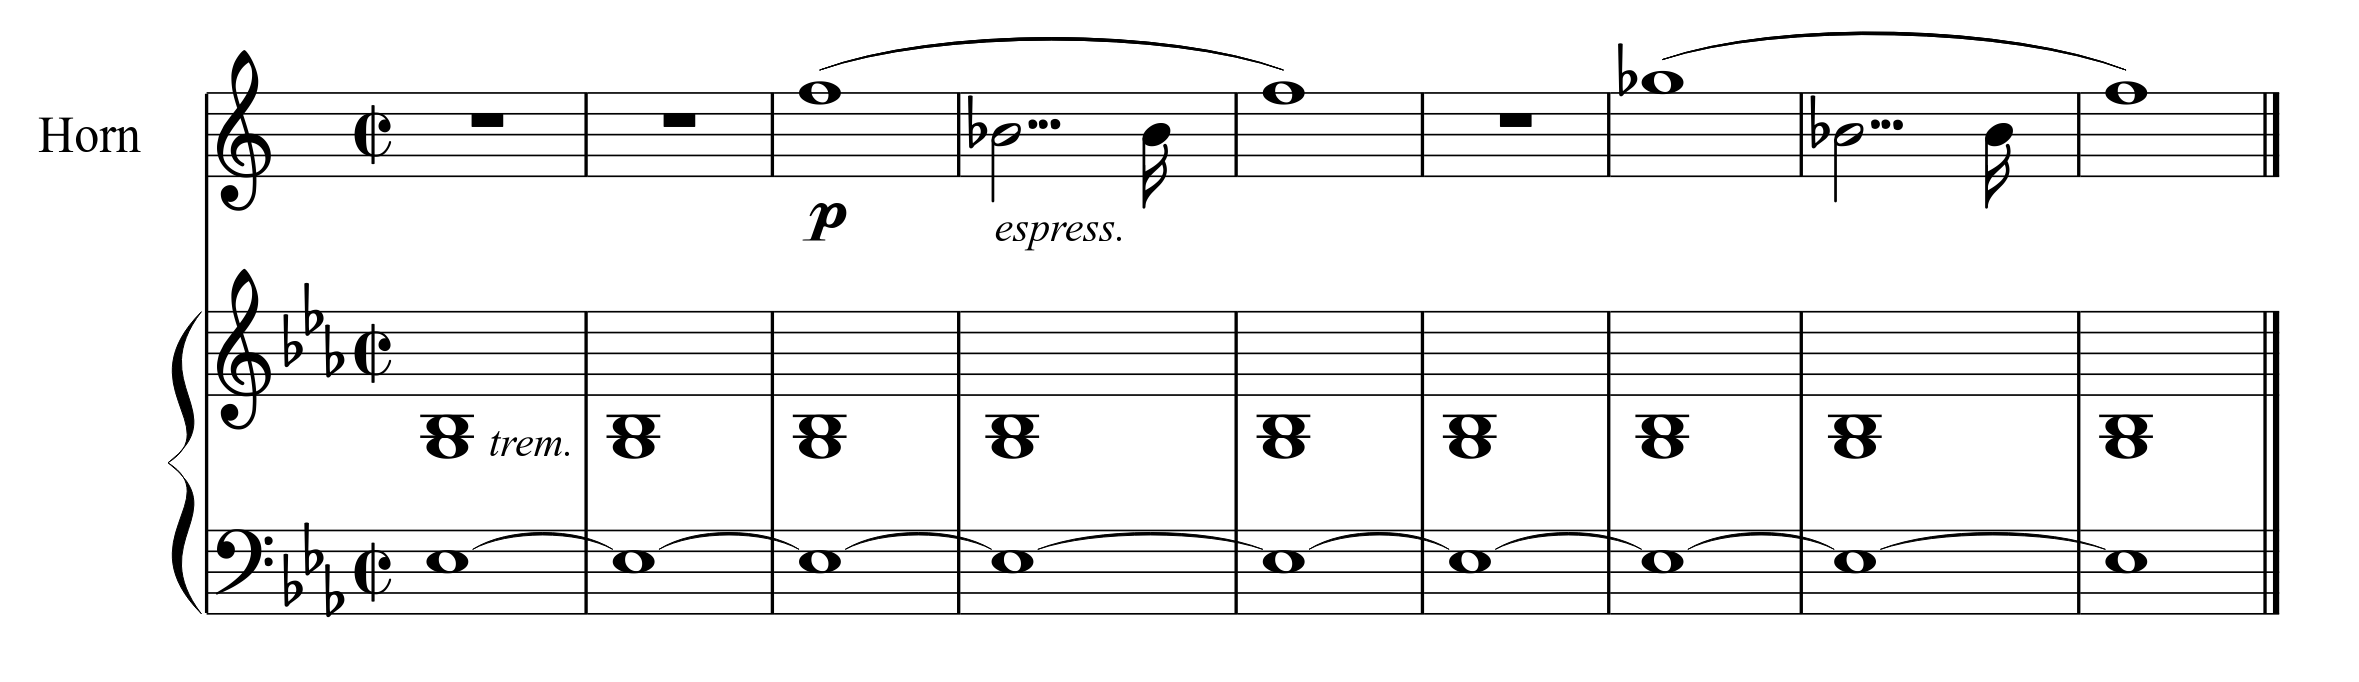
\includegraphics[scale=0.2]{bruckner4a}\caption{Bruckner Symphony No.4 first movement opening call}
\label{fig:bruckner1a}
\end{figure}

The orchestration is majestic and the thematic writing is conversational with relatively simple themes toggling back and forth between woodwind, brass and strings. 

%theme at C in first movement with counter theme%

A two quarter, triplet quarter theme with cross-wise motion is also extremely declamatory.

\begin{figure}[H]
\centering
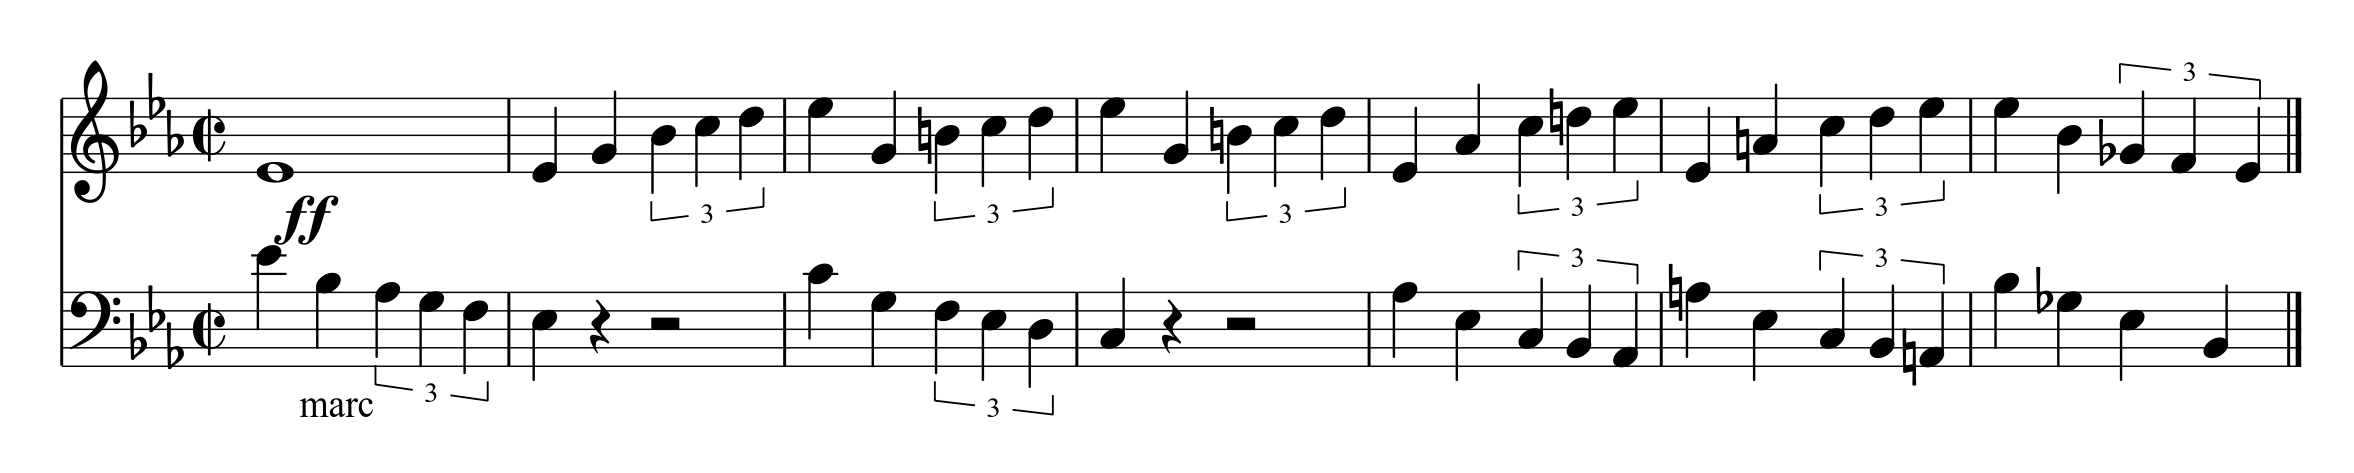
\includegraphics[scale=0.2]{bruckner4b}\caption{Bruckner Symphony No.4 mvt1 declamatory theme}
\label{fig:bruckner1b}
\end{figure}

But there are some very lyrical moments where Bruckner relaxes the mood somewhat. 

\begin{figure}[H]
\centering
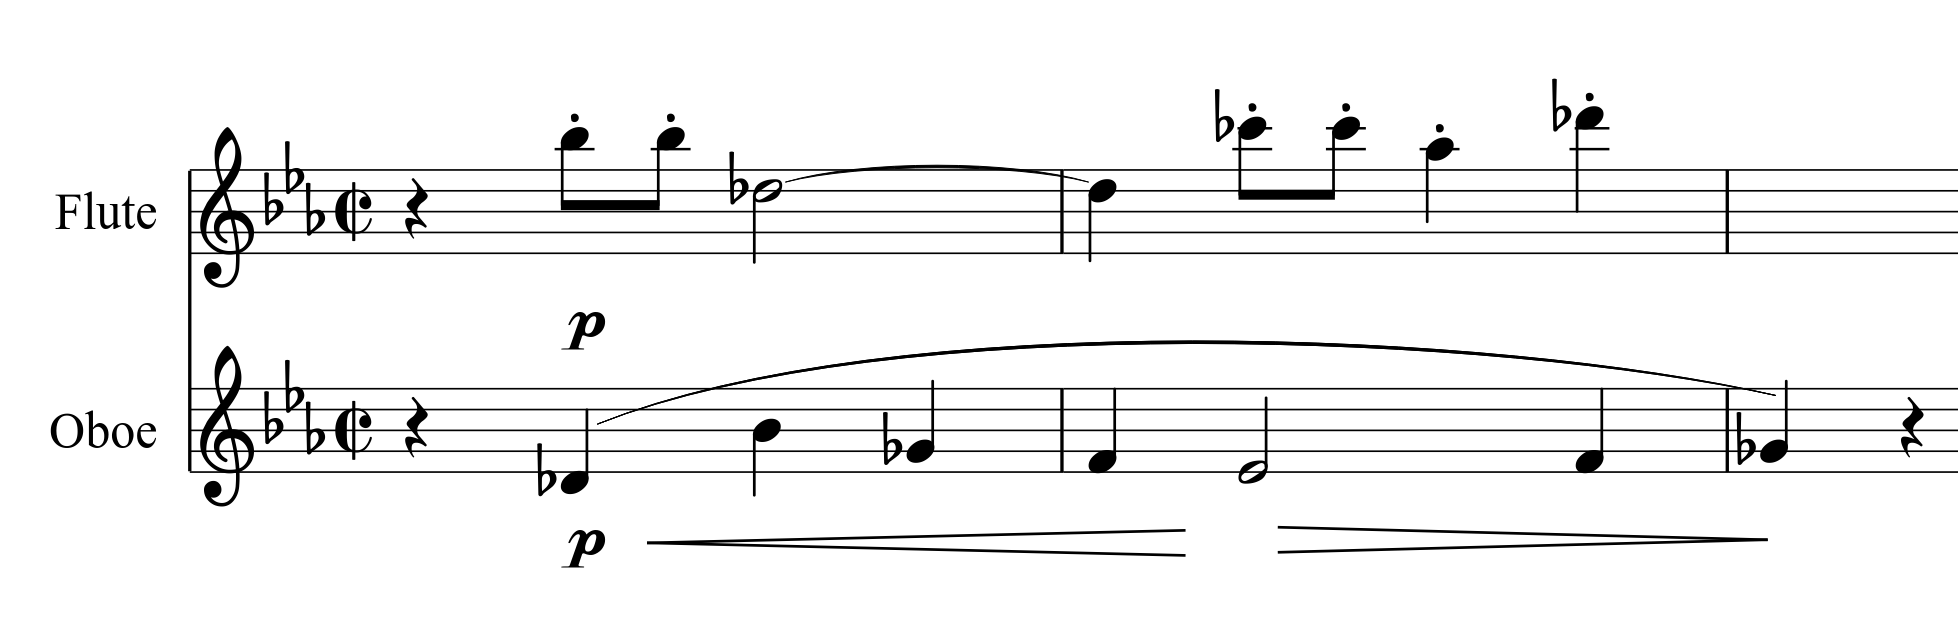
\includegraphics[scale=0.2]{bruckner4c}\caption{Bruckner Symphony No.4 mvt1 lyrical counterpoint}
\label{fig:bruckner1c}
\end{figure}

Bruckner takes great liberties with unison and octave melodic lines. 
Sections contrast and grate against each other like granite slabs (note the changes before figure G in the first movement). G itself is quite operatic in its suggestiveness. The thematic play is block against block with transposition and orchestration the only development at time. (Compare the later Jeux where themes are intricately similar but different). Despite the relative difficulty in creating a hierachy of thematic material in the exposition, the movement is in sonata form (with development at bar 193, figure M and recapitulation at bar 365, figure M and a coda at bar 501). 

\subsection{Second movement}

The second movement is also in sonata form. The movement begins in C minor with the cellos playing the main theme. Just as in the quieter moments of the first movement the timpani play a huge role in maintaining the background. In places, the brass harmonies hint at Wagner. Finally around figure M, Bruckner decorates his harmonies with more intense string writing. However, the movement always seems to be hanging on the edge; frail, despite the huge horn calls. 

The two main themes from this movement are: 
\begin{figure}[H]
\centering
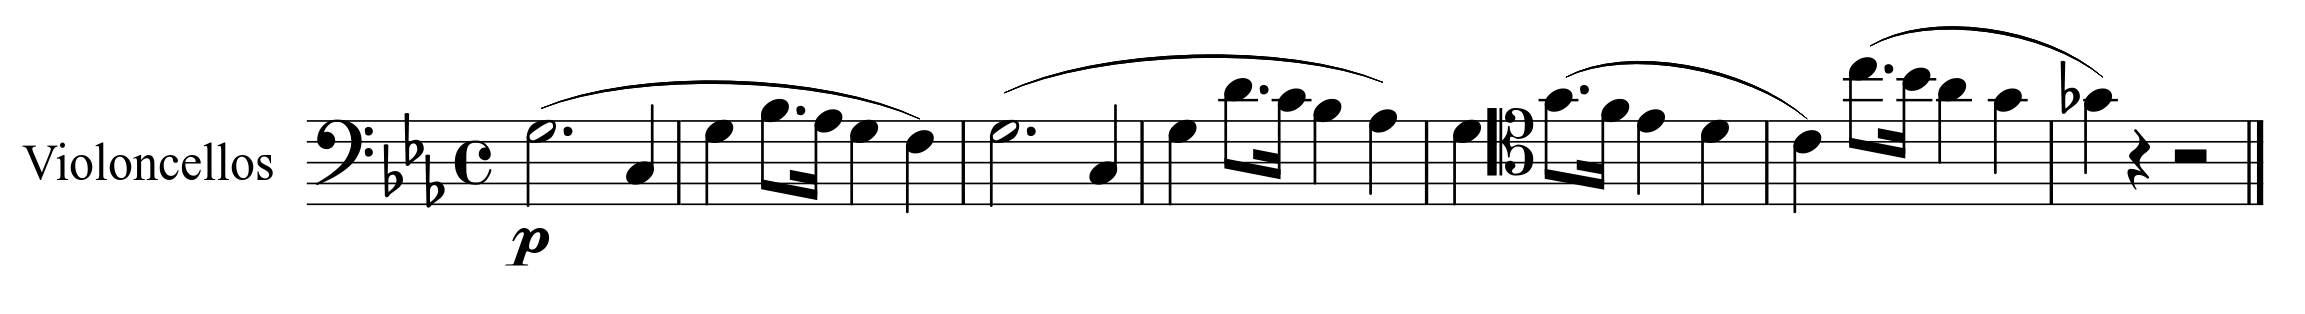
\includegraphics[scale=0.2]{bruckner4d}\caption{Bruckner Symphony No.4 mvt2 opening string theme}
\label{fig:bruckner1c}
\end{figure}

and

\begin{figure}[H]
\centering
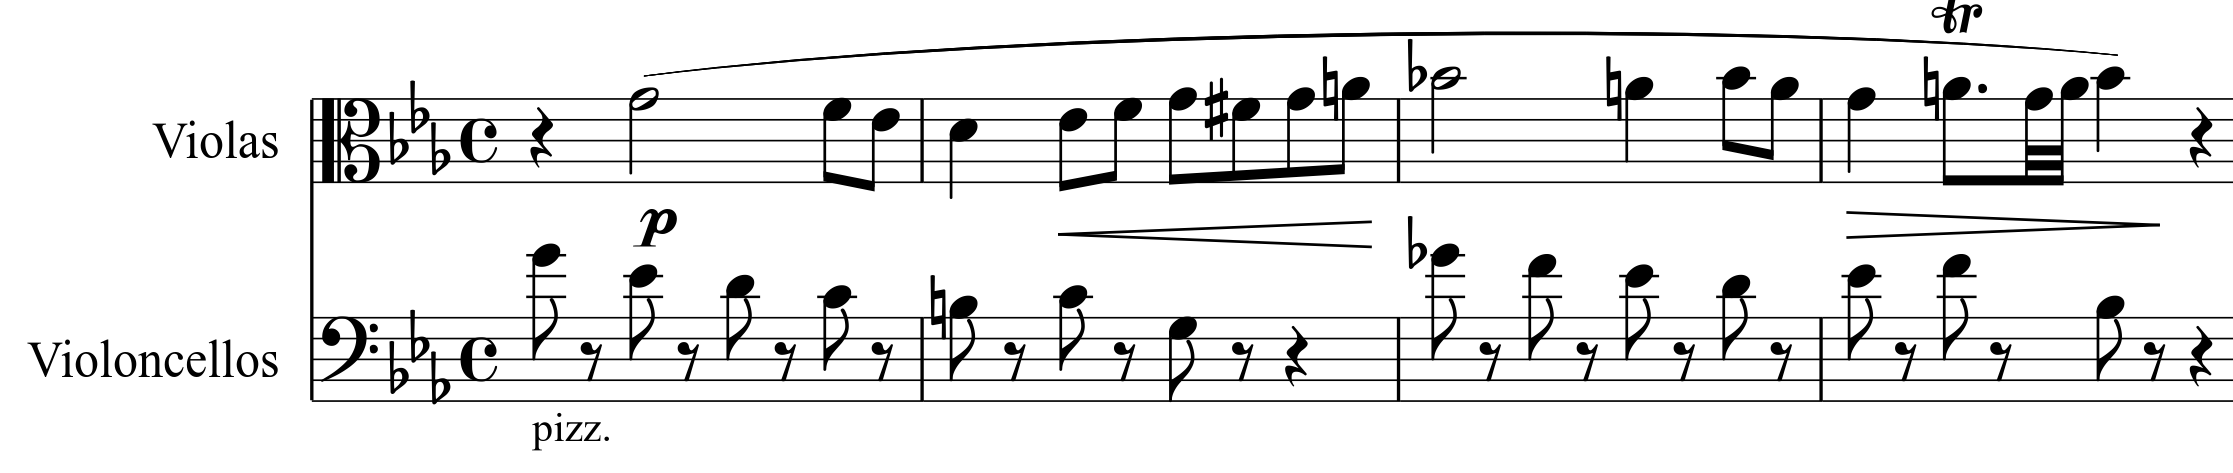
\includegraphics[scale=0.2]{bruckner4e}\caption{Bruckner Symphony No.4 mvt2 lyrical theme}
\label{fig:bruckner1c}
\end{figure}

\subsection{Third movement}

This movement clearly wares its hunting call on its sleeve. Typical of Bruckner too that we arrive at one glorious crescendo moment and the next passage is back in the meadows; light and airy. All the thematic material comprises larger intervals (4ths and 5ths). As tension builds by sequence, Bruckner uses more pedal points in this movement. The trio has a very Mahler-like feel to it. Clearly they both knew each other's work. Whilst Mahler started writing symphonies in 1888, working voraciously averaging one symphony every two years, Bruckner's themes and bravura style must have been appreciated by his colleague; so too his wunderhorn-like melodies. (Compare the first symphony with its L\"andler and themes from \textit{Lieder eines fahrenden Gesellen}.) The pastoral description is common to both composers.  

\subsection{Fourth movement}

Picking up where the third movement left off, on a B$\flat$, the fourth movement seems almost like a continuation of the third. Back has come the 2-quarter 3-triplet-quarter hammer motif from the first movement. Naturally the B$\flat$ is the dominant of E$\flat$ at bar 79. Quickly we are back to something much more cheeky which modulated aggressively through the keys. Figure F again uses tonic, submediant harmonies.  The introduction recurs at 203 and again leads to a large climax but this movement has perhaps spent itself somewhere before the close such is its tumultuous and never-ending shift of pace. 

Bruckner shares material amongst the movements which gives the work an overall homogeneous feel (although at well over an hour to play, perhaps a little tiresome). 




\chapter{Opera}
\label{opera}

\section{Opera post Beethoven}
Beethoven, Weber, Verdi, Wagner - Tristan and Ring. 

%%%%%%%%%
%Refer back to previous material but add musical examples
%%%%%%%%%


\section{Romanticism and Puccini: La Boh\`eme}
\begin{itemize}
\item Listen: \url{https://www.youtube.com/watch?v=ntg9vXxAia8}
\item Score: \url{http://imslp.org/wiki/La_boh%C3%A8me_%28Puccini,_Giacomo%29}
\item Reading (not for comment): \url{http://www.pittsburghopera.org/files/file/Study%20Guide%20for%20La%20boheme.pdf}
\end{itemize}

Giacomo Puccini was born into a musical family. Puccini's father was an organist and teacher. Puccini was the fifth of eight children, five girls, three boys. As Puccini learned his trade, his composition teacher introduced him to Verdi's scores (\textit{Rigoletto}, \textit{La traviata}). And from hearing \textit{A\"ida} he began to compose less for the organ. Puccini continued his studies in Milan under the tutelage of Antonio Bazzini beginning in 1880, also with Amilcare Ponchielli. He was joined in Milan by Pietro Mascagni, composer of \textit{Cavalleria Rusticana} (1890), an opera that started the \textit{Verismo} tradition (emphasis upon realism). In 1883 Puccini composed a ten minute orchestral piece, \textit{Capriccio Sinfonico}. Already operatic in nature; dramatic and poignant, one  can hear the beginnings of his phrase structure, the mood swings and the swirling, haunting melodies. The whole work sounds like an introduction and in a way, it is perhaps an overture to larger things. And then all of a sudden we hear the opening of \textit{La Boheme}. 

Just as `getting signed' today is key to success, so it was back then and the two main publishers were Ricordi and Lucca. After two less well known pieces \textit{Le villi} and \textit{Edgar} with libretti by Fernando Fontana, Ricordi commissioned new work and Puccini went through librettist after librettist. It seems Puccini was very picky about who he worked with eventually siding with Giuseppe Giacosa and Luigi Illica. This opera was \textit{Manon Lescaut}. It is interesting to note that Illica and Giacosa were to remain faithful to Puccini for future successful operas. \textit{Manon Lescaut} was completed in 1892 after three years hard work. Immediately it has signature tenor lines and languorous phrasing. Recitative and Aria have disappeared as has a post-Verdi accompanimental style. 

The success of \textit{Manon Lescaut} now set Puccini fair financially. 

\textit{La boh\`eme} comes from Henri M\"urger's Sc\`enes de la vie de boh\`eme. Bohemianism is associated with carefree, gypsy-like lifestyle. There is a relatively intense history pertaining to the emergence of Puccini's version. It seems composers and publishers were all scrambling to the same story. Moreover, the libretto's gestation was lengthy and revised many times. Once the libretto was in good shape, Puccini worked on the score: 1895 saw the completion of the music. The premiere was set for Teatro Regiio, Turin; date 1st February 1896. Despite recommendations for conductors from Puccini, Ricodi selected young conductor Auturo Toscanini.

To top it all, \textit{La boh\`eme} received mixed reviews. 

\subsection{Synopsis}
The Opera is set in the Latin Quarter of Paris around 1830. Four artists are living a poor life. Rodolfo (poet), Marcello (painter), Schaunard (musician) and Colline (philosopher). They are ``Bohemians'', penniless but passionate about life. It's Christmas Eve and three of the men leave the flat to go to the cafe, leaving Rodolfo behind. Enter Mimi, frail, delicate (and ill) to ask for a candle. Love lights up the room. They eventually join the group at the cafe along with Musetta who, accompanied by her much older admirer Alcindoro tempts her ex, Marcello to fall in love with Musetta again. 

A month later. Mimi finds Marcello to tell him that Rudolfo, in a fit of jealousy has left her. When Marcello questions Rodolofo, he explains his departure was due to the fact he can not support her as she is dying (of consumption - TB). Mimi overhears this conversation but they meet and love, once again endures. Marcello and Musetta - now living together - also argue. 

In the fourth act, Marcello and Rudolfo are lamenting love. They are both separated from their loved ones. Schaunard and Colline try to brighten the atmosphere but the merriment is arrested when Musetta arrives with a dying Mimi. The friends go off to search for a doctor leaving Rudolfo and Mimi together. 

\subsection{What makes La Boh\`eme ground-breaking?}
Look at a review from critic of the time Eduard Hanslick (1825-1904)
\begin{quotation}
The few earlier operas that deal seriously with affairs between wanton courtesans and weak youths (\textit{La Traviata, Camen}, and most recently \textit{Manon}) have at least dressed them in picturesque national or historic garb, or set them in romantic surroundings and thus raised them out of the lowest regions of everyday wretchedness. With \textit{La Boh\`eme} our composers take the last step towards the naked, prosaic dissoluteness of our time: heroes in loud-checked trousers, gaudy ties and crumpled felt hats, cigarette butts in their mouths, their companions in bonnets and scanty shawls. This is new, a sensational break with the last romantic and artistic traditions of opera.
\end{quotation}

There's a new, more visceral depiction of everyday life. But amidst the mundane there are moments of pure poetry. In particular note the difference between the words of Mimi when she says, `actually my name is Lucia'. 

\subsection{Musical details}

The opening bravura theme comes from the earlier \textit{Capriccio Sinfonico}. 

\begin{figure}[H]
\centering
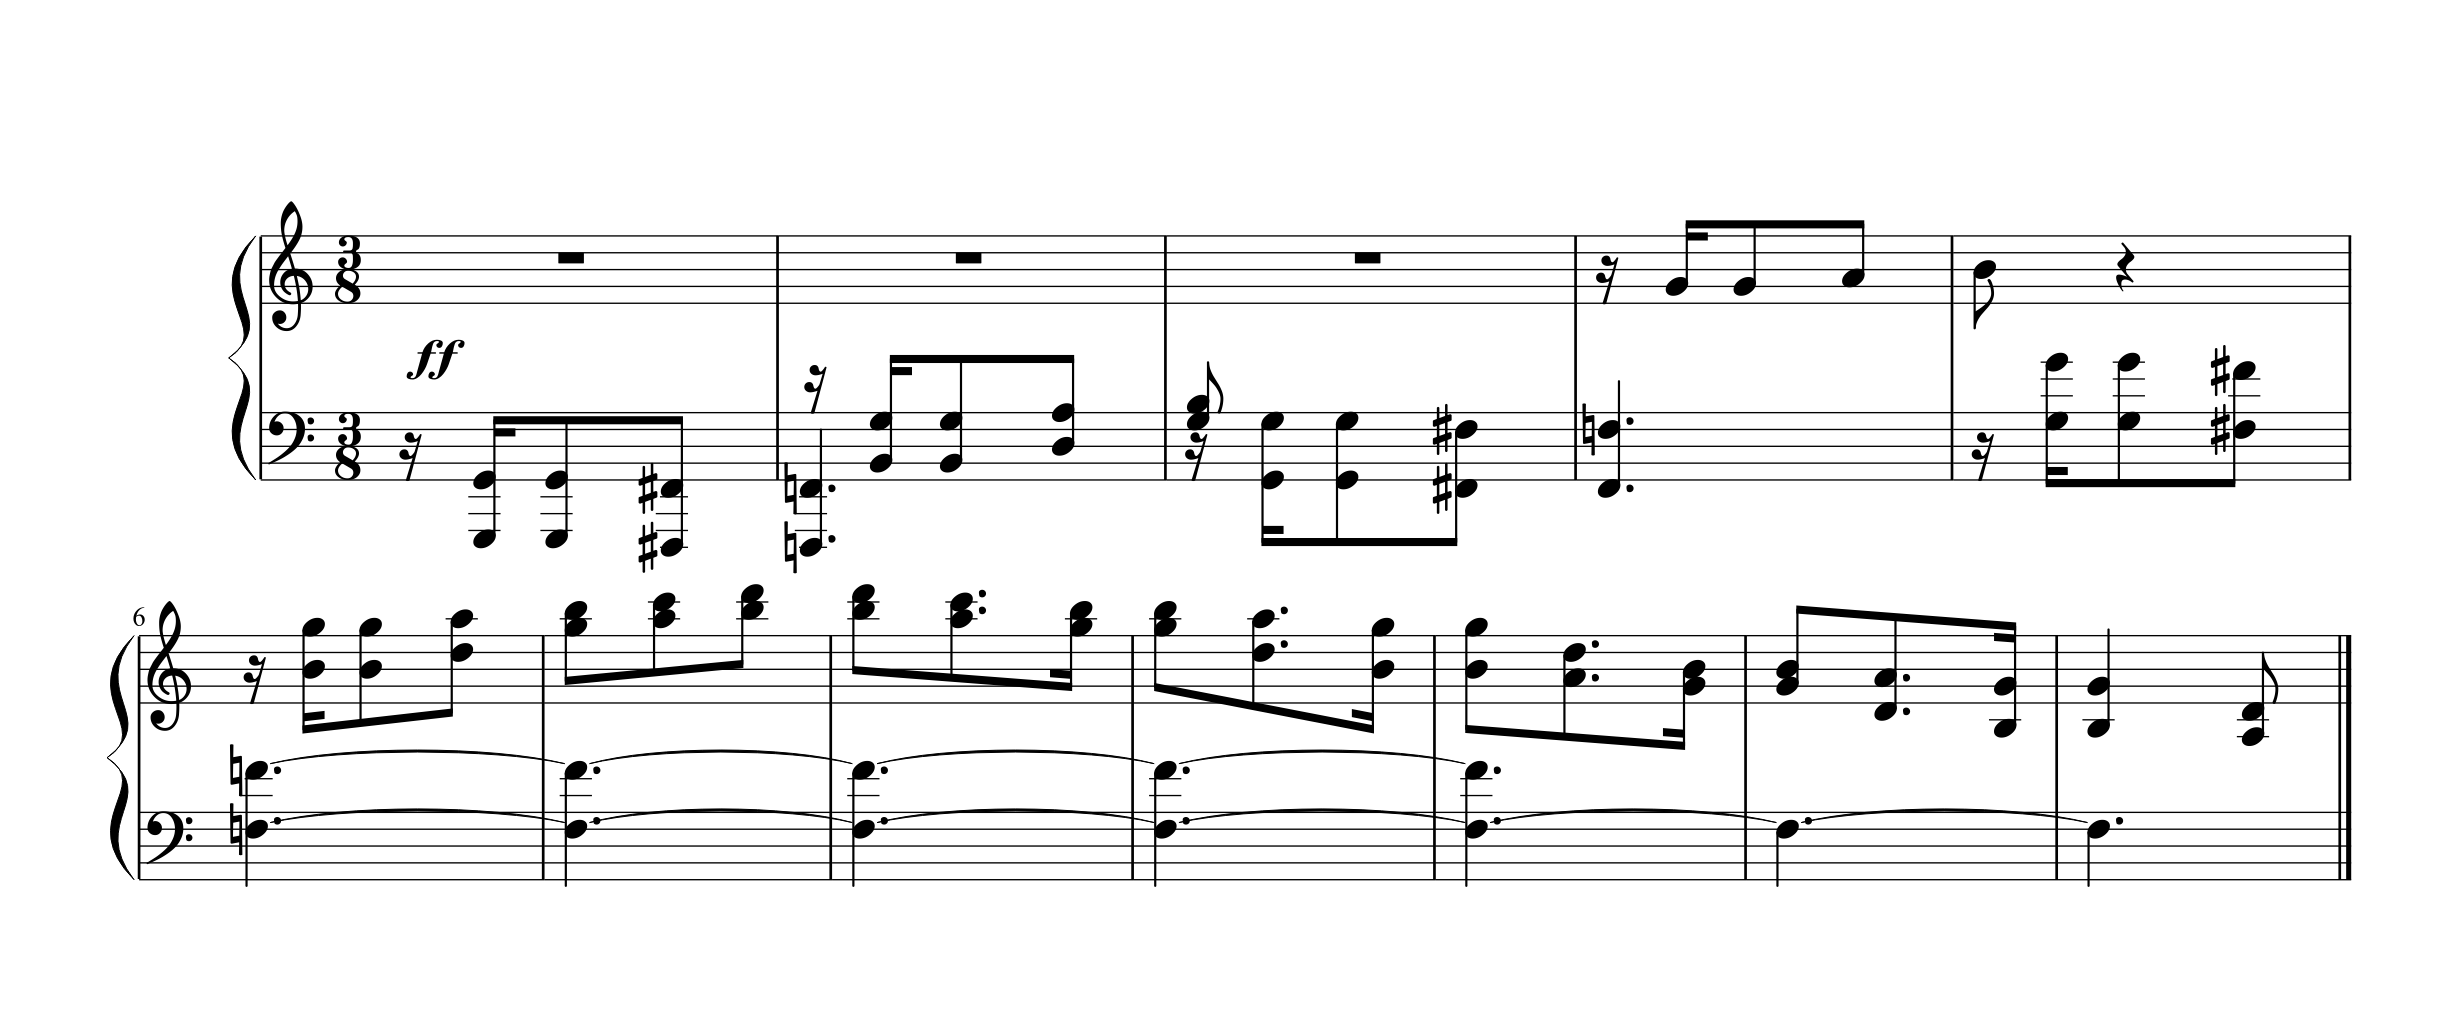
\includegraphics[scale=0.2]{boheme1}\caption{La Boh\`eme opening moments}
\label{fig:boheme1}
\end{figure}

Rodolfo's theme is a plaintive call swaying through high notes.

\begin{figure}[H]
\centering
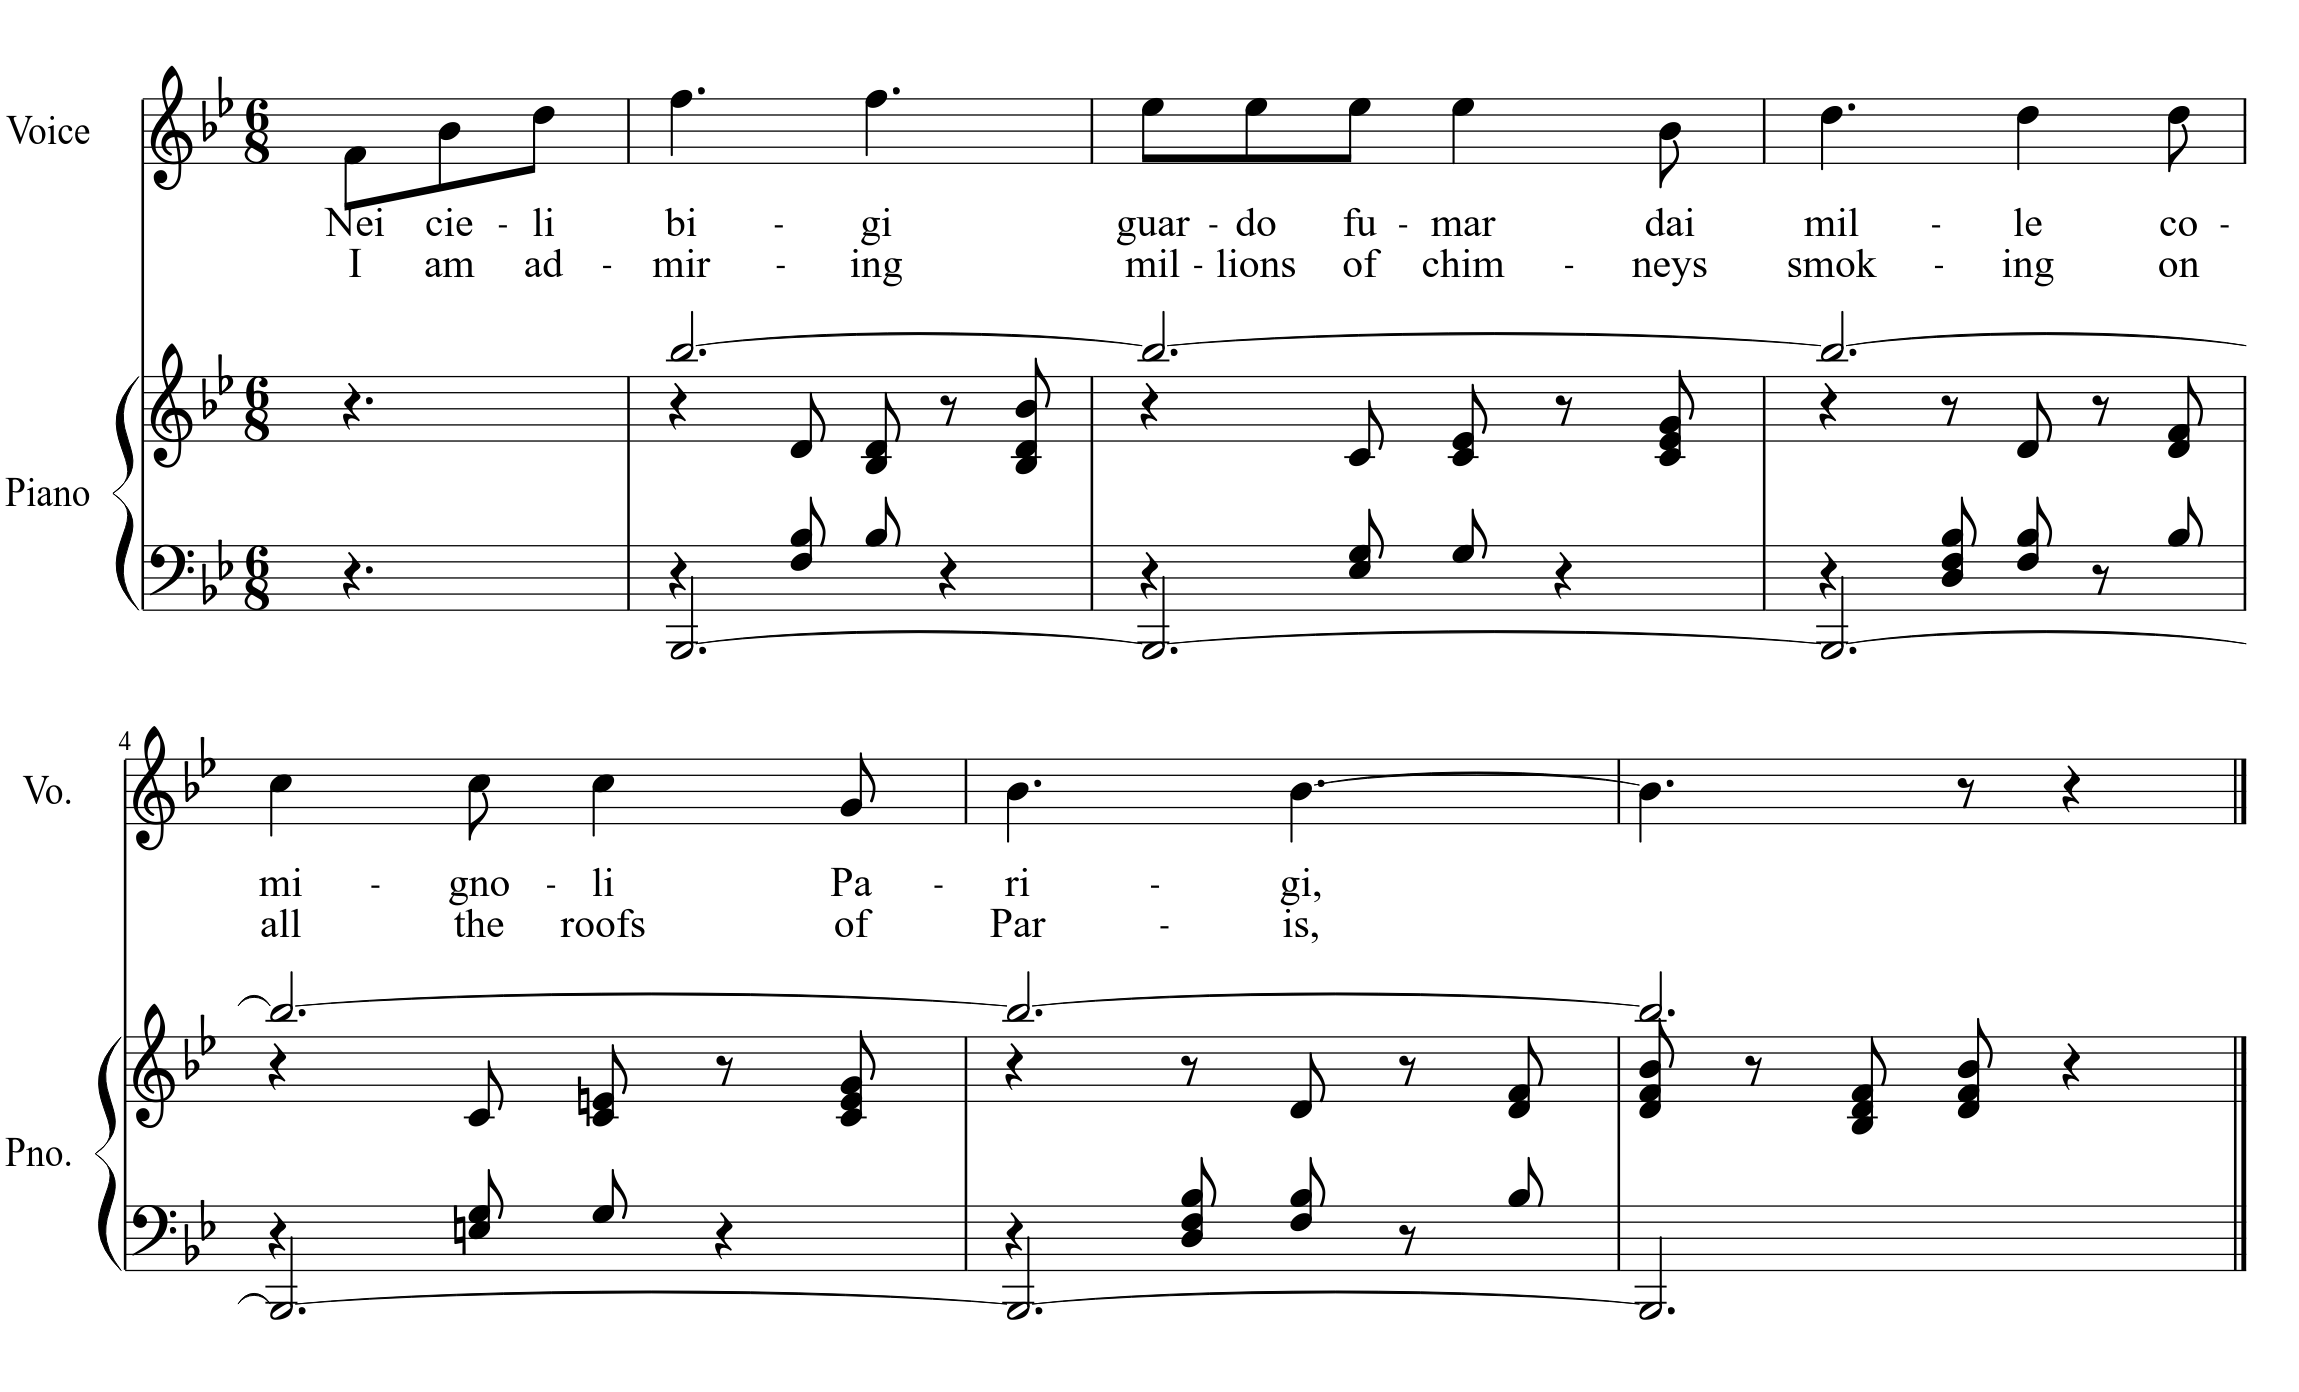
\includegraphics[scale=0.2]{rodolfotheme}\caption{Rodolfo's theme}
\label{fig:rodolfotheme}
\end{figure}
 
The themes are simple but poignant. Note Rodolfo's melody as he and Mimi search for the lost key. This tune could not be easier to remember but its falling (and subsequent climb-fall repeats) represents their forlorn love. 

\begin{figure}[H]
\centering
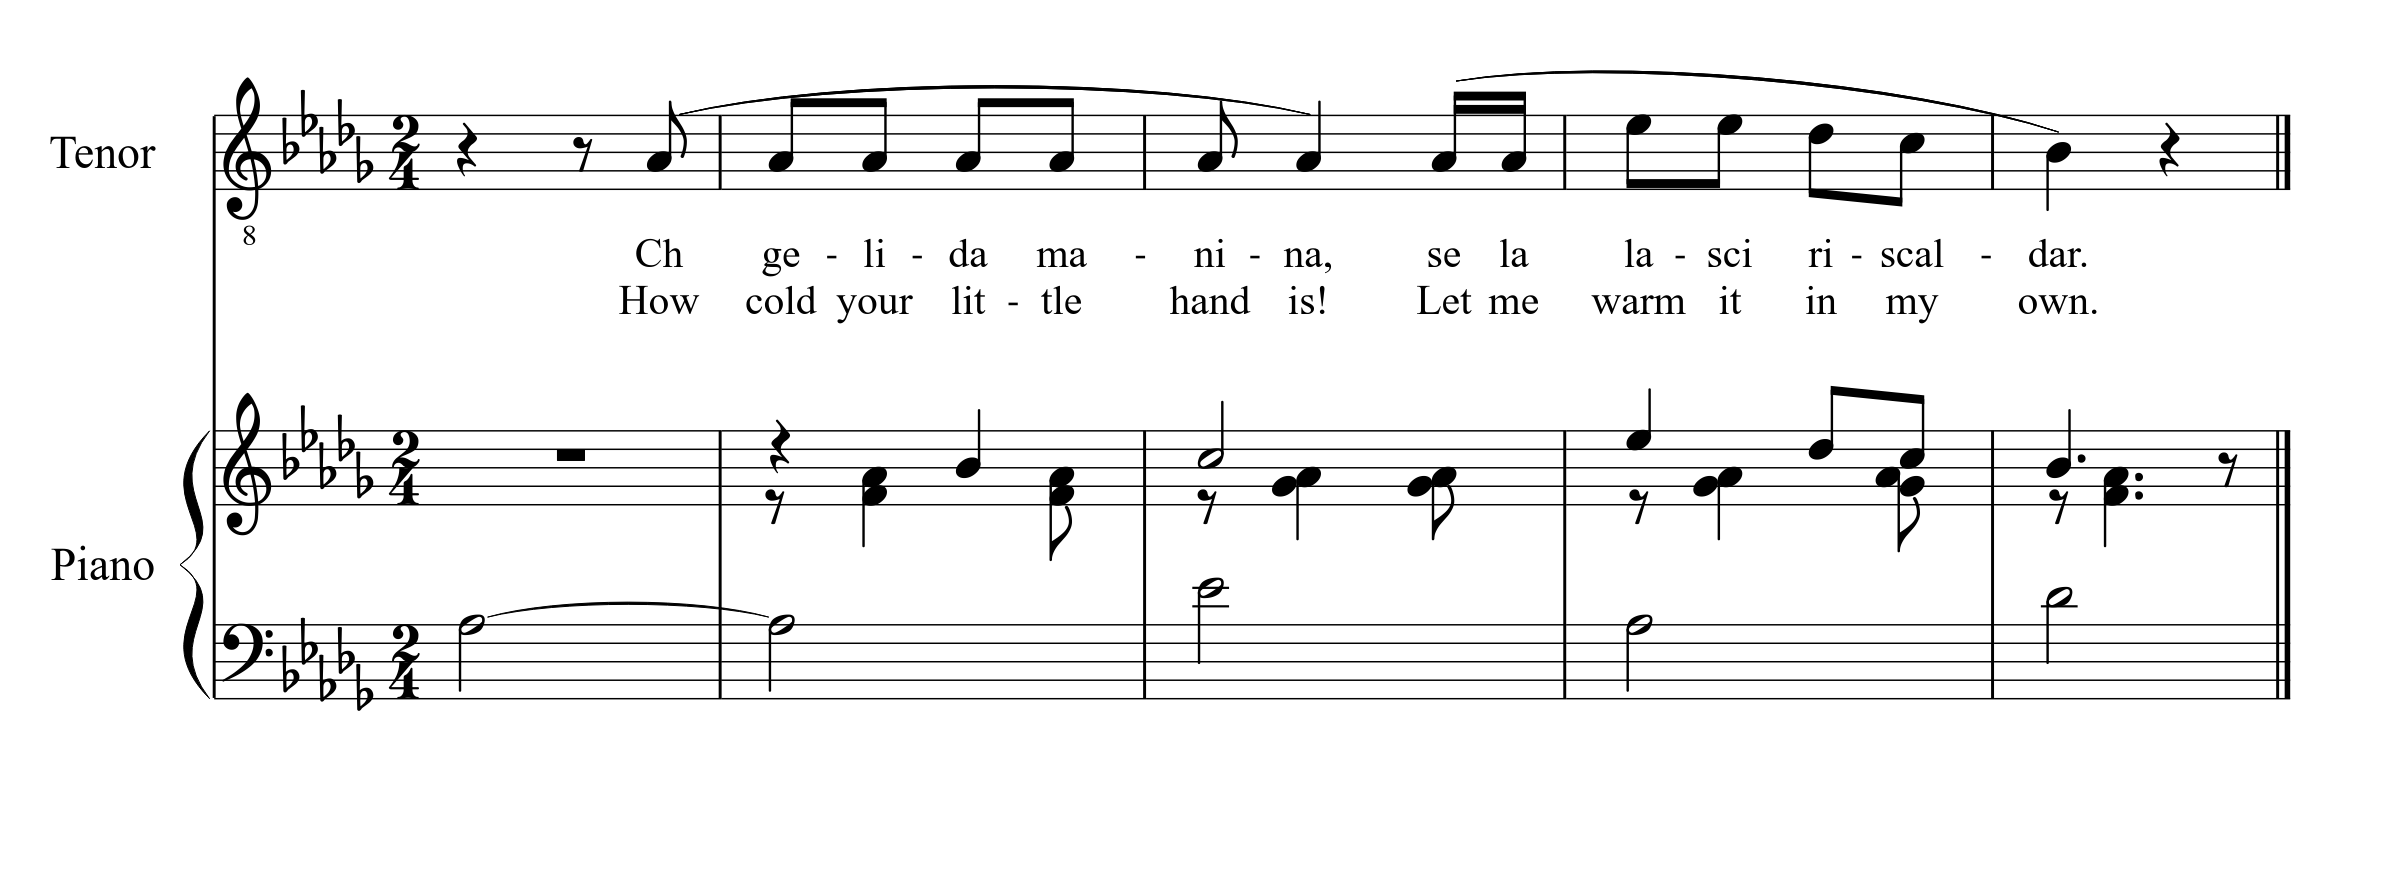
\includegraphics[scale=0.2]{rodolfokey}\caption{Rodolfo's key theme}
\label{fig:rodolfokey}
\end{figure}

Act II is the `Quatier Latin' and the boisterous atmosphere is represented by bristling parallel chords. 

\begin{figure}[H]
\centering
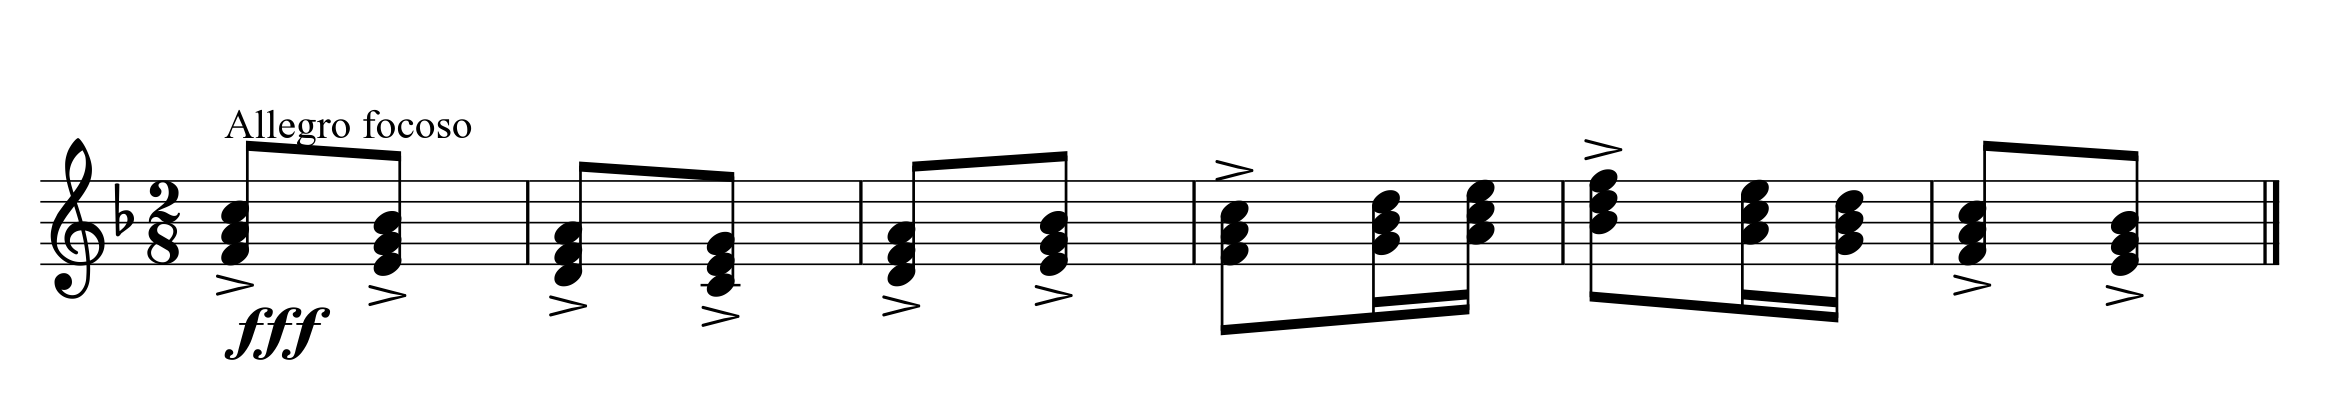
\includegraphics[scale=0.2]{quatierlatin}\caption{Quatier Latin opening}
\label{fig:quatierlatin}
\end{figure}

To add to the reality we see the arrival of toy maker Parpignol. The contrast of themes, and story-lines (Mimi and Rudolfo, Marcello and Musetta, Parpignol and children) again shows how Puccini is filling his bar with real life.

And with real tunes too! Musetta's solemn waltz theme had its original outing at a ceremony launching a battelship at Genoa. Hard to believe but it could easily be a whistled tune. 

\begin{figure}[H]
\centering
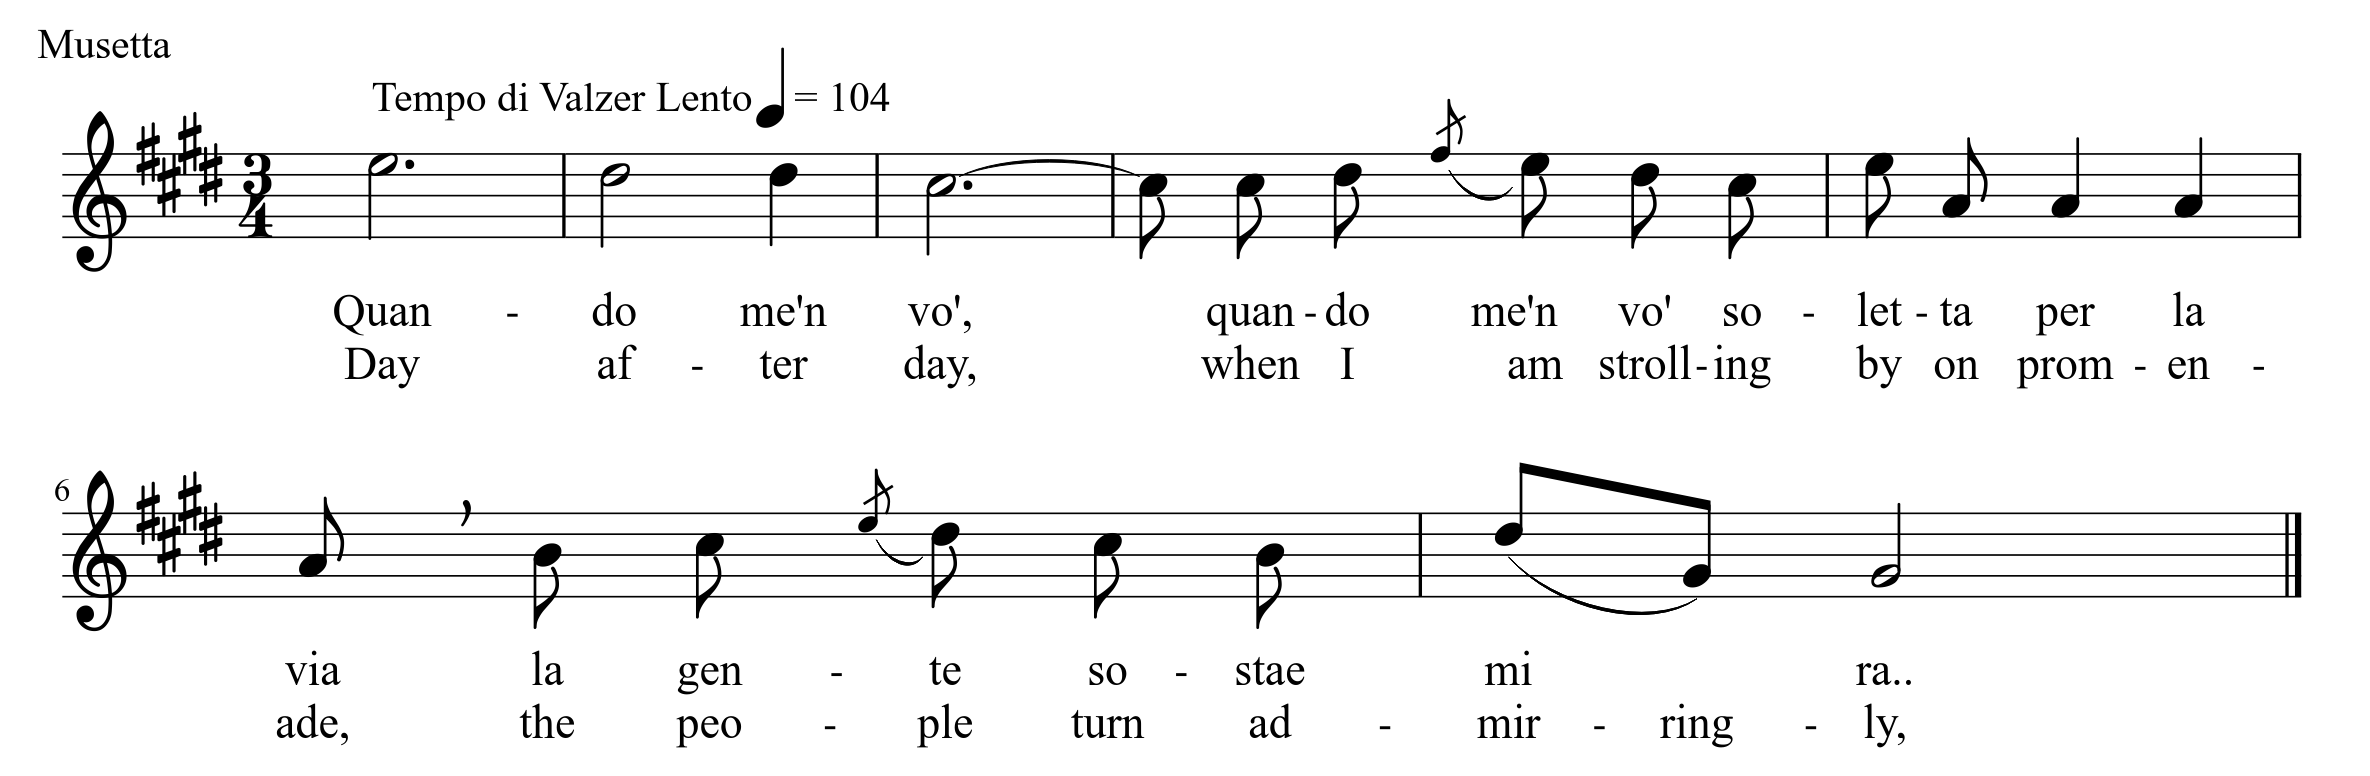
\includegraphics[scale=0.2]{musettatheme}\caption{Musetta's theme}
\label{fig:musettatheme}
\end{figure}

The story, by Henry Murger was published in paperback in 1851 and sold quickly and is autobiographical in nature. The opera attempts to be faithful to the story and the play that followed it. It is a highly sentimental tug at the heart-strings but it reaches out and touches everyone. Compare Puccini and Leoncavallo's treatment of the same theme. 

And of course, if that wasn't enough for Puccini, he continued with \textit{Tosca} (after a play by Victorien Sardou (1831-1908)). The play itself has a torrid history of production and interesting antecedents.

For Puccini, getting around to writing the opera was a long process. There were many premieres of \textit{La Boh\`eme} to attend. Imagine the scene, 5th October 1897. A performance of \textit{La Boh\`eme} in Vienna with Mahler in attendance. Apparently there were too many little children in the Quatier Latin scene and Mahler's laughter, Puccini never forgot.   

\textit{Tosca} has all the ingredients of a tragic opera: Love, betrayal, death between the three key characters; Tosca, Cavaradossi and Scarpia. The scene is Rome, 1800. It does have some of the most intense confrontation scenes in Italian opera and the last scene of Act 1 was well used in Quantum of Solace. The characterisation and the opportunity for highly expressive singing (something 19/20th Century singers must have relished as they propelled themselves to stardom) is there in spades. Perhaps for the tenor (Cavaradossi) it has to be the aria `E lucevan le stelle' early into act III. 

The rest is history. Madame Butterfly - first performed in 1904 and based upon the one act play by David Belasco, itself a dramatisation of a story by John Luther Long, La fanciulla del West, La rondine, a triptych of operas including Gianni Schicchi and of course, Turandot.
  









 

\chapter{Ballet Music}
\label{balletmusic}

%\section{Scores}

\section{Impressionism and Debussy: Jeux}
\begin{itemize}
\item Listen: \url{https://www.youtube.com/watch?v=eT9ZQEZQSXs}
\item Score: \url{http://imslp.org/wiki/Jeux_%28Debussy,_Claude%29}
\item Reading: \url{http://adrian-moore.staff.shef.ac.uk/teaching/mus126/debussy_jeux_eimert.pdf}
\end{itemize}

Claude Debussy (1864-1918) brings much of what we know of impressionism in painting to the musical score. Easy to say but perhaps more difficult to define. Debussy was friends with painters such as James Whistler (1834-1903). When Whistler moved to Paris in 1855 he rented a studio in the Latin Quarter (bohemianism). His later work is very impressionistic and adopts the title Nocturne used explicitly to depict the obscure.      
Debussy was also heavily influenced by writers of the time such as Paul Verlaine (1844-1896) and St\'ephane Mallarm\'e, both symbolist writers. Symbolism focused naturally upon symbols and as a result dislocated itself from reality. As a consequence themes revolved around spirituality and the darker parts of the imagination, easily rendered through symbols (such as ravens (Poe)). 

Mallarm\'e's poem from 1876 \textit{Pr\'elude \`a l'apr\`es-midi d'un faune} was taken by Debussy for his orchestral prelude of the same name, composed in 1894 (see table~\ref{tab:faune}). Mallarm\'e was obsessed with the musical in words and indeed wrote a sonnet to Wagner. 

\begin{figure}[H]
\centering
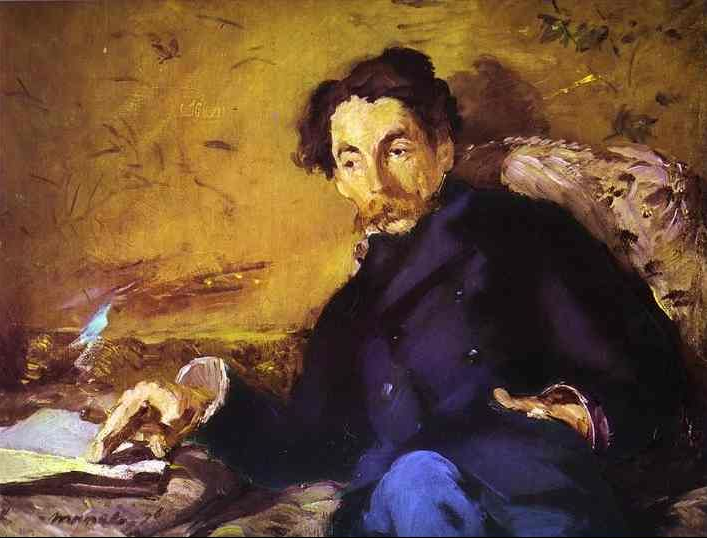
\includegraphics[scale=0.2]{manetmalarme}\caption{St\'ephane Mallarm\'e by Edouard Manet (1876)}
\label{fig:quatierlatin}
\end{figure}

\begin{table}[h!]
\begin{tabular}{|l|l|} \hline
Le Faune: & \\
Ces nymphes, je les veux perp\'etuer. & These nymphs that I would perpetuate: \\
Si clair, & so clear \\
Leur incarnat l\'eger, qu'il voltige dans l'air & And light, their carnation, that it floats in the air  \\
Assoupi de sommeils touffus. & Heavy with leafy slumbers. \\
Aimai-je un r\^eve? & Did I love a dream? \\
Mon doute, amas de nuit ancienne, s'ach\`eve & My doubt, night’s ancient hoard, pursues its theme \\
En maint rameau subtil, qui, demeur\'e les vrais & In branching labyrinths, which being still \\
Bois m\^eme, prouve, h\'elas! que bien seul je m'offrais & The veritable woods themselves, alas, reveal \\
Pour triomphe la faute id\'eale de roses. & My triumph as the ideal fault of roses. \\
R\'efl\'echissons… & Consider… \\
ou si les femmes dont tu gloses & if the women of your glosses \\
Figurent un souhait de tes sens fabuleux! & Are phantoms of your fabulous desires! \\
Faune, l'illusion s'\'echappe des yeux bleus & Faun, the illusion flees from the cold, blue eyes \\
Et froids, comme une source en pleurs, de la plus chaste: & Of the chaster nymph like a fountain gushing tears: \\
Mais, l'autre tout soupirs, dis-tu qu'elle contraste & But the other, all in sighs, you say, compares \\
Comme brise du jour chaude dans ta toison? & To a hot wind through the fleece that blows at noon? \\
Que non! par l'immobile et lasse p\^amoison & No! through the motionless and weary swoon \\
Suffoquant de chaleurs le matin frais s'il lutte, & Of stifling heat that suffocates the morning, \\
Ne murmure point d'eau que ne verse ma fl\^ute & Save from my flute, no waters murmuring \\
Au bosquet arros\'e d'accords; et le seul vent & In harmony flow out into the groves; \\
Hors des deux tuyaux prompt \`a s'exhaler avant & And the only wind on the horizon no ripple moves, \\
Qu'il disperse le son dans une pluie aride, & Exhaled from my twin pipes and swift to drain \\
C'est, \`a l'horizon pas remu\'e d'une ride & The melody in arid drifts of rain, \\
Le visible et serein souffle artificiel & Is the visible, serene and fictive air \\
De l'inspiration, qui regagne le ciel. & Of inspiration rising as if in prayer. \\

\hline
\end{tabular}
\caption{Opening of \textit{Pr\'elude \`a l'apr\`es-midi d'un faune}}
\label{tab:faune}
\end{table}

Debussy achieved success early into his student days. He entered the Paris Conservatoire in 1873 for 11 years of study. It was here that Debussy first heard Wagner's early operatic output. He continued to study with C\'esar Franck and Ernest Guiraud. He was awarded the Premier Grand Prix de Rome in 1884 for his cantata \textit{L'Enfant prodigue} (the prodigal son). Debussy was 21. You can already hear the development of phrases and the growth of romantic harmonies. But this was a hasty work, written in a month and apparently in the style of Massenet so as to please the judges of the Prix de Rome. 

As winner of the prize (which continues to this day), Debussy set off for Rome in 1885. And clearly at this time Wagner remained a huge influence (though as an master, not necessarily as one to model). Around the turn of the decade, Wagner dominated French culture, particularly literary culture.

Both in literary circles and in music, symbolism highlighted the sensuous. Colour took on greater significance. With the darkness of war (Franco-Prussian and ultimately WWI), artists wanted to re-inject colour into the world. But equally at that time, the Russian nationalist composers were beginning to influence European composers. The great exhibitions (such as the World Fair of 1889) saw Rimsky-Korsakov conduct two concerts of Russian music. Out of this melting pot arose Debussy's early works. 

Debussy also knew Brahms and had visited and dined with him on a number of occasions. But one of his more substantial friendly relationships was with composer Erik Satie.

\subsection{Works}
Although you will probably know Debussy best by his ballet works, it is his opera \textit{Pell\'eas et M\'elisande} that should be heard more frequently. It occupied Debussy's 30s for around ten years. \textit{Pell\'eas et M\'elisande} is a play by Maurice Maeterlink (1862-1949) written around 1893. Debussy's opera received its premiere in 1902. 

And after Nocturnes (1899) subtitled: \textit{Nuages} (clouds), \textit{F\^etes} (Festivals) and \textit{Sir\'enes} (Sirens) Debussy naturally turned to the sea with \textit{La Mer} (1903-05). We know of Debussy's intent through letters to his publisher Auguste Durand. Debussy's personal life was one of turmoil at the time too. He left his first wife, Lily, who shot herself in the heart (and survived) and took up with one Mme Emma Barda, the wife of a wealthy banker. 

Although Debussy's orchestral colour is unsurpassed, to understand his musical syntax one must go to the piano pieces. These are extraordinarily difficult to play but Debussy wrote pieces of varying technical difficulty and the `Children's Corner' pieces are excellent works to study. The first volume of \textit{Images pour piano} (1904-05) deliver that archetypal impressionistic sound that one might imagine when looking at the works of Monet (The Water-Lily Pond of 1899). And indeed are laced with titles such as \textit{Reflets dans l'eau}. The second set of \href{http://petrucci.mus.auth.gr/imglnks/usimg/4/4a/IMSLP254485-PMLP02391-Debussy__Claude-Images_2e_Serie_pour_Piano_seul_Durand_6994_scan.pdf}{\textit{Images}} is more complex, and is set over three staves. \textit{Cloches à travers les feuilles} (Bells through the leaves - and clear use of the whole-tone scale), \textit{Et la lune descend sur le temple qui fut} And the moon descends on the temple that was, and \textit{Poissons d'or} Golden fish. 

But it is the later works where Debussy is really experimental. The second set of Pr\`eludes becomes ever more dissonant. And in Debussy's orchestral ballet masterpiece, \textit{Jeux} (1912) we hear very detailed construction. 

\subsection{Ballets Russes and Sergei Diaghilev}
This was a time of great impresarios (Sergei Diaghilev 1872 - 1929), great choreographers (Michel Fokine 1880-1942) and even greater ballet dancers (Vaslav Nijinsky 1889 - 1950). It was clear that around 1910, ballet's maestros were no less self-absorbed. Stravinsky and Debussy were often misunderstood by Fokine and Benois (designer) who were much more involved with the day-to-day running of the company (a company which worked and toured extremely hard). 

The first dress rehearsals for \textit{Jeux} were agonising. Costumes designed by L\'eon Bakst were inappropriate and Diaghilev altered them himself. But Diaghilev was working on \textit{Jeux} and \textit{The Rite of Spring} at the same time. The opening night was 15th May 1913. The ballet is your typical `fumble in the dark' - or as outlined to the audience at the premiere:

\begin{quotation}
The scene is a garden at dusk; a tennis ball has been lost; a boy and two girls are searching for it. The artificial light of the large electric lamps shedding fantastic rays about them suggests the idea of childish games: they play hide and seek, they try to catch one another, they quarrel, they sulk without cause. The night is warm, the sky is bathed in pale light; they embrace. But the spell is broken by another tennis ball thrown in mischievously by an unknown hand. Surprised and alarmed, the boy and girls disappear into the nocturnal depths of the garden.
\end{quotation}

Nijinsky was disheartened at the reaction to \textit{Jeux} which was not riotous but lacklustre. Debussy, writing to a friend shortly after the premiere was dismayed at Nijinsky's approach which bordered (negatively) on the Dalcrozian (eurhythmics - approaching music through movement). 

%%continue with ballet stuff and the rite
%%emphasise the importance of the Eimert text

\subsection{The Eimert text}
The Eimert text was written in 1957 in a small but incredibly important German publication called `Die Reihe'. Eimert focuses first upon the originality of Debussy's score. Debussy clearly wrote pure music but also a number of pieces that were collaborative and \textit{Jeux} is no exception. Perhaps a quick comparison to the music for D'Annunzio's mystery play \textit{Le martyre de saint S\`bastien} might shed light upon \textit{Jeux's} originality. The music from 1911 is wholeheartedly romantic in nature. \textit{Jeux} then, might easily be heard as Debussy trying again to free his technical palette. Moreover, we should be careful to pigeon hole \textit{Jeux} as impressionist (symbolist perhaps). Debussy himself said of \textit{Images} and Eimert makes a point of suggesting this is even truer of \textit{Jeux} is `I am trying to introduce something new - realities, so to speak. What idiots call ``impressionism'''. Eimert proceeds to make an astute rendering of the musical score, highlighting Debussy's never-ending inventiveness.  

\section{The power of the new}
\begin{itemize}
\item \href{http://www.nytimes.com/2012/09/19/arts/music/radical-music-sometimes-shocking-sometimes-subtle.html?pagewanted=all&_r=0}{NY Times article}
\end{itemize}

\section{Modernism and Stravinsky: The Rite of Spring}
\begin{itemize}
\item Listen: \url{https://www.youtube.com/watch?v=rq1q6u3mLSM}
\item Listen: \url{https://www.youtube.com/watch?v=ewOBXph0hP4}
\item Score: \url{http://imslp.org/wiki/The_Rite_of_Spring_%28Stravinsky,_Igor%29}
\item Reading: Hill, P. (2000). Stravinsky: \textit{The Rite of Spring.} Cambridge Music Handbooks. Cambridge University Press
\item Online: \href{http://publishing.cdlib.org/ucpressebooks/view?docId=ft967nb647;brand=ucpress}{Stravinsky and the Rite of Spring: The Beginnings of a Musical Language, Pieter C. van den Toorn. 1987. University of California Press}

\end{itemize}

\begin{figure}[H]
\centering
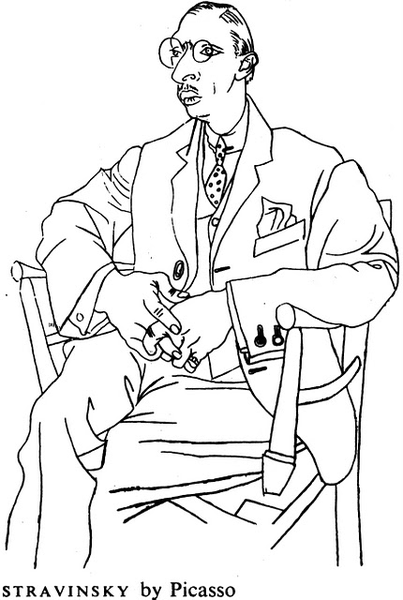
\includegraphics[scale=0.2]{Stravinsky_picasso}\caption{Stravinsky by Picasso}
\label{fig:stravpicasso}
\end{figure}

We have this account of Debussy and Stravinsky playing the four-hand piano version of the Rite. Indeed the piano duet version of the Rite was published in 1913, the year of the premiere; the full orchestral score was not published until 1921. The advantage of the piano version is that the orchestra is removed. The score is naked and we can hear all the dissonance and rhythmic complexity. 

Stravinsky's first collaboration with Diaghilev was \textit{The Firebird}. Diaghilev's original choice of composer was Liadov (Diaghilev's old harmony tutor) and when he showed no interest Diaghilev turned to the pupil of Rimsky-Korsakov, Stravinsky. There is a moment when, in December 1909 Diaghilev telephones Stravinsky to offer him the commission and Stravinsky attests to having already begun the work. 


Diaghilev was inspried by Wagner but was less interested in the financial outlay required to stage opera so focused upon ballet. After \textit{Firebird} came \textit{Petrushka} in 1911. (Diaghilev had had great success with a ballet set to Rimsky-Korsakov's \textit{Sch\'eh\'erazade} and was clearly a proponent of new music). Stravinsky was paid 1500 roubles for \textit{The Firebird} and due to its success, he knew there would be further opportunities. And it was at this point that Stravinsky began to think about the \textit{Rite}. As he wrote to the painter Roerich:

\begin{quotation}
Naturally, the success of \textit{The Firebird} has encouraged Diahilev for future projects, and sooner of later we will have to tell him about the `Great Sacrifice'....As soon as I said that I was working with you, both Diaghilev and Bakst were delighted, Bakst saying he thught our idea was a noble one. They were greatly relieved, obviously, to hear that my secret did not concern Benois: Diaghilev would have been greatly offended if Benois had been involved.
\end{quotation}

In the Summer of 1910, Diaghilev and Nijinsky arrived at Stravinsky's studio and instead of hearing early work on the \textit{Rite} got a new composition: \textit{Petrushka}. Petrushka was a Russian version of Punch. 

We should also remember that Ravel, the great orchestrator had been commissioned by Diaghilev in 1908 to write \textit{Daphnis et Chlo\'e} a ballet of huge proportions. Diaghilev was, at this time almost bankrupt but was still commissioning work. 

It was Diaghilev's aspiration for greatness that led to this outpouring of new music. By 1910 he was looking to form his own company and was waiting for the time when Nijinsky would begin to choreograph his own movement. (Until this time Fokine was doing this). But Nijinsky began to take control as he sketched steps to Debussy's \textit{L'Apre\`es-midi d'un faune}. As Stravinsky wrote to his mother in April 1912:

\begin{quotation}
Diaghileve and Nijinsky are mad about my new child, \textit{Le Sacre du printemps.} The unpleasant part is that it will have to be done by Fokin whom I consider an exhausted artist, one who has travelled his road quickly and who writes himself out with each new work. \textit{Sch\'eh\'erazade} was the high point of his achievement and, consequently, the beginning of his decline.
\end{quotation}

Fokine left the company in June that 1912 and Nijinsky danced \textit{La Sacre du printemps} at the Th\`e\^atre des Champs-\'Elys\'ees on 29 May 1913. Diaghilev, ever the conjourer of spetacle had given free tickets to young artists and fans. Thus was the melting pot set: the rich and famous seated in their boxes; the unruly standing up. Diaghilev had the house lights turned up at the change of scene and the police were called in to remove the most unruly. Both Ravel and Delius were present at the premiere. The ballet company continued apace, the music set its place in history. 

\begin{figure}[H]
\centering
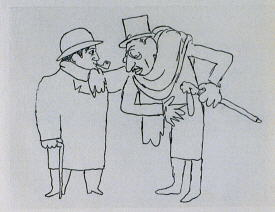
\includegraphics[scale=1.0]{picassostrav_cocteau}\caption{Stravinsky and Picasso by Jean Cocteau}
\label{fig:stravpicasso_cocteau}
\end{figure}

Stravinsky went on to write \textit{Les noces}, \textit{Pulcinella} and \textit{Apollo} amongst a career of over 60 years of composing.  

Peter Hill's key text accounts for some of the folk music `borrowings'. The opening bassoon line was the only tune Stravinsky acknowledged to be of folk origins. Harmonically the \textit{Rite} is brutal. Triads are superposed. 

\begin{figure}[H]
\centering
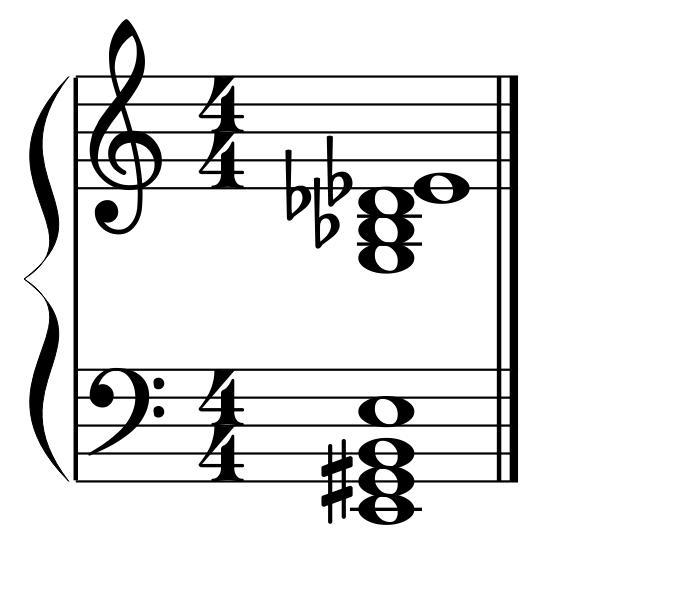
\includegraphics[scale=0.15]{augurschord}\caption{Augurs of Spring}
\label{fig:augurschord}
\end{figure}

The octotonic scale is used (see pages 44 and on in Hill). Hill talks about minor tetrachords (a four note combination) that is the first four notes of a minor scale (Tone, Semi-tone, Tone). Note this use in Ritual of the Rival Tribes.

\begin{figure}[H]
\centering
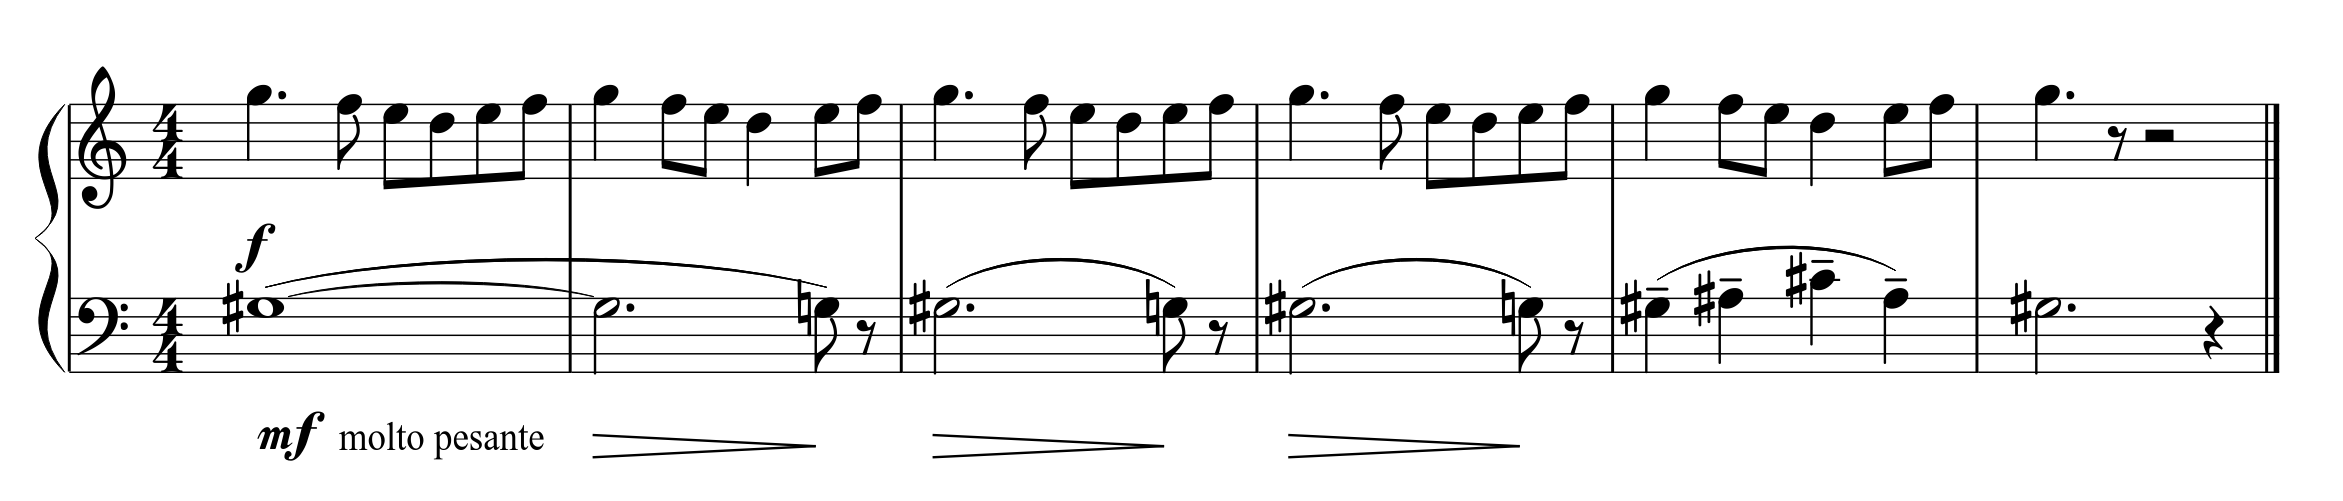
\includegraphics[scale=0.2]{rivaltribes}\caption{Ritual of the Rival Tribes}
\label{fig:rivaltribes}
\end{figure}

It will be worth commenting upon the music's main moments - in particular the use of ostinato in various numbers and the continuing development of rhythm. Having listened to the piano version it will also be useful to look at orchestration. 






\chapter{Expressionism and Serialism}
\label{twentieth}

Although serialism here is mentioned it really only appears rigorously in the Webern example. 
Prior to this we see two pieces by Webern's colleagues, Schoenberg and Berg.
Both use the voice; both are highly expressionistic in nature. 


\section{Schoenberg: Pierrot Lunaire}
\begin{itemize}
\item Listen: \url{https://www.youtube.com/watch?v=N-zW10__i4M}
\item Score: \url{http://imslp.org/wiki/Pierrot_Lunaire,_Op.21_%28Schoenberg,_Arnold%29}
\item Reading: \url{http://www.jstor.org/stable/pdfplus/10.2307/832890.pdf}
\end{itemize}

Expressionism began in paint through artists such as Franz Marc, Emil Nolde and Vasily Kandinsky. Marc and Kandinsky are associated with the \textit{Blaue Reiter} movement though Nolde is better associated with \textit{Die Br\"uke} - the Bridge, a similar group of expressionist artists. Primitive arts and the expressive use of colour triggered an emotional search for the spiritual. Kandinsky's \textit{Der Blaue Reiter} of 1903 gave the group its name. Schoenberg was a member of this group being as he was both an accomplished musician and painter. Although \textit{Der Blaue Reiter} sought the spiritual, it moved towards the abstract (note a gradual move towards cubist tendencies), the subjective (introspective) and the avant-garde. 

Thus, Schoenberg's early works develop the idea of `going beyond'. 

\textit{Verkl\"arte Nacht (Transfigured Night)} from 1899 is inspired by a poem by Richard Dehmel of the same name. 

\begin{table}[h!]
\begin{tabular}{|l|l|} \hline
Zwei Menschen gehn durch kahlen, kalten Hain; & Two people are walking through a bare, cold wood;\\
der Mond l\"auft mit, sie schaun hinein. & the moon keeps pace with them and draws their gaze.\\
Der Mond l\"auft über hohe Eichen; & The moon moves along above tall oak trees,\\
kein W\"olkchen tr\"ubt das Himmelslicht, & there is no wisp of cloud to obscure the radiance\\
in das die schwarzen Zacken reichen. & to which the black, jagged tips reach up.\\
Die Stimme eines Weibes spricht: & A woman’s voice speaks:\\	  	
\hline
``Ich trag ein Kind, und nit von Dir, & ``I am carrying a child, and not by you.\\
ich geh in S\"unde neben Dir. & I am walking here with you in a state of sin.\\
Ich hab mich schwer an mir vergangen. & I have offended grievously against myself.\\
Ich glaubte nicht mehr an ein Gl\"uck & I despaired of happiness,\\
\hline
und hatte doch ein schwer Verlangen & and yet I still felt a grievous longing\\
nach Lebensinhalt, nach Muttergl\"uck & for life’s fullness, for a mother’s joys	\\
\hline
und Pflicht; da hab ich mich erfrecht, & and duties; and so I sinned,\\
da lie{\ss} ich schaudernd mein Geschlecht & and so I yielded, shuddering, my sex\\
von einem fremden Mann umfangen, & to the embrace of a stranger,\\
und hab mich noch daf\"ur gesegnet. & and even thought myself blessed.\\
Nun hat das Leben sich ger\"acht: & Now life  has taken its revenge,\\
nun bin ich Dir, o Dir, begegnet.'' & and I have met you, met you.'' \\	
\hline
Sie geht mit ungelenkem Schritt. & She walks on, stumbling.\\
Sie schaut empor; der Mond l\"auft mit. &  She looks up; the moon keeps pace.\\
Ihr dunkler Blick ertrinkt in Licht. & Her dark gaze drowns in light.\\
Die Stimme eines Mannes spricht: & A man’s voice speaks:\\
\hline
``Das Kind, das Du empfangen hast, & ``Do not let the child you have conceived\\
sei Deiner Seele keine Last, & be a burden on your soul.\\
o sieh, wie klar das Weltall schimmert!  & Look, how brightly the universe shines!\\
Es ist ein Glanz um alles her; & Splendour falls on everything around,\\
Du treibst mit mir auf kaltem Meer, & you are voyaging with me on a cold sea,\\
doch eine eigne W\"arme flimmert & but there is the glow of an inner warmth\\
von Dir in mich, von mir in Dich. & from you in me, from me in you.\\
Die wird das fremde Kind verkl\"ren, & That warmth will transfigure the stranger’s child,\\
Du wirst es mir, von mir geb\"ren; & and you bear it me, begot by me\\
Du hast den Glanz in mich gebracht, & You have transfused me with splendour,\\
Du hast mich selbst zum Kind gemacht''. & you have made a child of me.''\\
\hline
Er fa{\ss}t sie um die starken H\"uften. & He puts an arm about her strong hips.\\
Ihr Atem k\"u{\ss}t sich in den L\"uften. & Their breath embraces in the air.\\
Zwei Menschen gehn durch hohe, helle Nacht. & Two people walk on through the high, bright night.\\
\hline
\end{tabular}
\caption{Verkl\"arte Nacht (Transfigured Night), Richard Dehmel}
\label{tab:faune}
\end{table}

It is scored for string sextet although there is a version for string orchestra. Its harmonies are clear but there is an increased chromatic contrapuntalism, inherited from Wagner and also heard in Mahler and Strauss. 
The poem is highly charged and this desire is reflected in the music through wrought melodies and rising sequences. 

A \textit{Pelleas und Melisande} followed in 1899. The Maeterlinck play (1893) was hugely popular at the time and its theme of love, jealousy and death played completely into the expressionist's hand. The music has grief-stricken passion with huge chords and vast changes of orchestral density. Schoenberg's \textit{Chamber Symphony no.1} pushed the boundaries of harmony even further and coincided with the writing of his treatise on harmony in 1910 (published in 1922). 

The \textit{Five Orchestral Pieces} Op.9 of 1909 is notable for the development of \textit{Klangfarbenmelodie} in particular in movement III: Farben. Only through orchestration does the music develop: there is hardly any melodic or rhythmic articulation. 

This pushing at the boundaries was noticed even by Schoenberg himself. Of his song-cycle \textit{Das Buch der hangenden Garten} Op.15 from 1910 he wrote, I have `broken through every restriction of a bygone aesthetic'. He explained that he had emancipated dissonance - that a chord could resolve this way and that and be equally acceptable. Debussy had done something similar with his non-functional harmony. 

\begin{figure}[H]
\centering
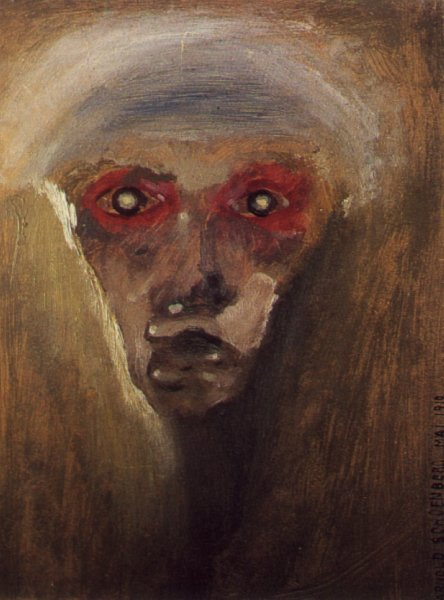
\includegraphics[scale=0.8]{roteblick}\caption{Der Rote Blick - the Red Gaze (1910)}
\label{fig:roteblick}
\end{figure}

Two music dramas followed in quick succession: \textit{Ewartung} (expectation) for soprano and orchestra (1909) and \textit{Die gl\"uckliche Hand} (the lucky hand) for voices and orchestra (1910/13). In \textit{Ewartung} we hear the hidden thoughts of a woman waiting in the forest for her lover (a Pelleas version again). The synopsis is as follows:

\begin{quotation} 
A woman is in an apprehensive state as she searches for her lover. In the darkness, she comes across what she first thinks is a body, but then realises is a tree-trunk. She is frightened and becomes more anxious as she cannot find the man she is looking for. She then finds a dead body, and sees that it is her lover. She calls out for assistance, but there is no response. She tries to revive him, and addresses him as if he were still alive, angrily charging him with being unfaithful to her. She then asks herself what she is to do with her life, as her lover is now dead. Finally, she wanders off alone into the night.
\end{quotation}

The madness of the tortured mind develops further still with \textit{Pierrot Lunaire} of 1912 for voice and small ensemble comprising piano, flute (pic), clarinet (bass), violin (viola) and cello. Whilst many note this piece as pivotal for its use of Sprechstimme (a kind of semi-pitched vocalisation) this piece projects Schoenberg's own fascination with (and suspiciousness of) numbers. 

\subsection{Pierrot Lunaire Op.21}

\url{http://www.lunanova.org/pierrot/index.html} for online texts and score animations. 

Who was Pierrot? Pierrot was a pantomime character and is commonly represented as a sad clown. Columbine is the object of his desires; Harlequin the object of hers. Thus again a love triangle with Pierrot originally the object of ridicule but during Symbolist times, the ultra-sensitive loner with only the moon for company.  

The structure of the work is as three times seven poems drawn from Albert Giraud's writings from 1884 (original in French with German translation by Otto Hartleben).  

\begin{table}[h!]
\begin{tabular}{|p{5.0cm}|p{5.0cm}|p{5.0cm}|} \hline
\textbf{Part One} & \textbf{Part Two} & \textbf{Part Three} \\\hline
Mondestrunken (Moondrunk) & Nacht (Passacaglia) (Night) & Heimweh (Homesickness)\\\hline
Columbine & Gebet an Pierrot (Prayer to Pierrot) & Gemeinheit! (Vulgarity)\\\hline
Der Dandy (The Dandy) & Raub (Theft)  & Parodie (Parody)\\\hline
Eine blasse W\"ascherin (An Ethereal Washerwoman) &  Rote Messe (Red Mass) & Der Mondfleck (The Moonspot)\\\hline
Valse de Chopin (Chopin Waltz) & Galgenlied (Gallows Song)  & Serenade\\\hline
Madonna & Enthauptung (Beheading) & Heimfahrt (Barcarole) (Homeward Bound)\\\hline
Der kranke Mond (The Sick Moon) & Die Kreuze (The Crosses) & O Alter Duft (O Ancient Fragrance)\\\hline
\end{tabular}
\caption{Pierrot Lunaire, 1912}
\label{tab:pierrot}
\end{table}

The stark rendition (especially when semi-staged) and the numerological references are well worth further investigation. 

As Schoenberg paired down the notational script of music so to did his works become more conceptual in size. 
His most famous students were Anton Webern and Alban Berg. Although Berg would follow his composition teacher down the serial road, he was always concerned with larger forms which serialism would not sustain. Webern however was not worried about this and as a consequence his complete oeuvre can be found on just three compact discs. 

Schoenberg's later works including the \textit{Variations for orchestra} (1926/28), \textit{Violin concerto} (1934/36), \textit{String quartet No. 4} (1936), \textit{Piano concerto} (1942), \textit{String Trio} (1946)
and the six minute \textit{A Survivor from Warsaw} (1947) are well worth following up. 
 
\section{Berg: Wozzeck}
\begin{itemize}
\item Listen: \url{https://www.youtube.com/watch?v=uUkbjO8dkDI}
\item Reading: \url{http://adrian-moore.staff.shef.ac.uk/teaching/mus126/wozzeck.pdf}
\end{itemize}

Useful text \textit{Anton von Webern} by Malcolm Hayes \citeyearpar{hayes1995anton}

Amongst numerous song cycles, key works of Alban Berg (1885-1935) to follow up are:
\begin{itemize}
\item Piano Sonata Op.1 (1907)
\item String quartet Op.3 (1910)
\item Wozzeck Op.7 (1914-22)
\item Lyric Suite (string quartet, 1925-6)
\item Lulu (1929-35)
\item Violin concerto (1935) 
\end{itemize}

Berg's early life was not a happy one. At age 18, his father had died, the family was poor, Alban's health was unsteady, he was not successful intellectually, he was unhappy in love yet had fathered an unwanted child. Berg considered suicide. 

Berg's early career was heading towards accountancy when he met Schoenberg. He learned his trades quickly and although poor, was gifted an inheritance in 1905 which allowed him to resign his government job in 1906. In Schoenberg's class Berg quickly became friends with Anton von Webern.

Musically Berg and Webern went separate ways: Berg looked to the past, Webern to an uncertain future, though both men knew the risks they were taking. Egon Wellesz recounts the premiere performance of Schoenberg's Op.10 quartet: (\href{http://conquest.imslp.info/files/imglnks/usimg/c/c1/IMSLP29725-PMLP66179-Schoenberg_-_SQ_No._2_score.pdf}{score})

\begin{quotation}
The atmosphere in the elegant and old-fashioned Boesendorfer Hall was tense from the beginning ... The first 
movement had hardly begun when, enraged by the unexpected C in the fifth bar, the music critic named Karpath 
jumped up from his seat and shouted, ``Stop it!'' Unperturbed, the Rose Quartet went on; but it was in that 
scherzo that, after a \textit{fortissimo}, the audience started laughing and its laughter drowned out the 
music. An elderly gentleman sitting in front of Mahler began whistling on a door key. I heard Mahler 
shouting, ``I'll risk five florins (the fine for disturbing the peace) and box you on the ear!'' ``You are 
not here as director of the Opera, you can't order me to stop,'' the man retorted. Mahler rose from his seat, 
but at that moment two young men, pupils of Schoenberg, rushed forward and carried the man out of the hall.
\citep[p32]{monson1979alban}
\end{quotation} 

We should be careful of Karen Monson's  regurgitation of this vignette however. The premiere of the second 
quartet was December 1908. Thing is, Mahler was in Europe until quite late in 1908, having returned from the 
US in April. He conducted concerts in May and September in Prague (the latter was the premiere of the 7th 
Symphony), then in Munich (27th Oct) and Hamburg (9th November). Getting close to 23rd Dec... but not close 
enough. By 29th November he was in New York where he stayed for the next few months. So, he was in Vienna 
while Schoenberg was finishing/revising Op. 10 and could certainly have heard it. But, he certainly knew it - 
in 1908 he ``warmly recommended it" to Richard Strauss (according to De La Grange \citeyearpar{de2007gustav}). 

By the summer of 1907 Berg had been studying harmony and counterpoint with Schoenberg for over two years and was ready to undertake original composition. After numerous small song cycles, Berg began his piano sonata: a planned three movements. Only one transpired and Schoenberg said that was enough. (\href{http://petrucci.mus.auth.gr/imglnks/usimg/7/75/IMSLP234327-SIBLEY1802.21900.4ff7-39087012041663score.pdf}{score})
For all its chromaticism this work is in sonata form and the key of Bminor. 

We should remind ourselves that Berg and Webern were composing at a time of huge Bruckner symphonies (the symphonies being around 10 years old), Strauss was writing virtuoso tone poems and Mahler was conducting his own symphonies. 
Berg was friends with the artist Gustav Klimt and Klimt was the Damien Hurst of his age. Experimentalism was certainly `in the air'.

Berg's first string quartet was premiered on April 24, 1911, just before his wedding to Helene Nahowski. At this point in his life he took his leave as student from Schoenberg. 

On May 3rd, 1911 he married Helene but finances were still tight. For work, Berg (who had been signed to Universal through solid success with the quartet) began copying parts and making piano reductions of scores (mainly Schoenberg's). Schoenberg was working on \textit{Gurrelieder}, the apogee of orchestral and choral forces - so grand it required a new kind of score paper to be produced. It is interesting to note Berg's (and to an extend Webern's) slavish duty to their master.  

Berg began work on a large scale piece based upon poems by his friend Peter Altenberg. The premiere of the \textit{Five Altenberg Lieder} was March 31, 1913. The Vienna scandal was as riotous as the Parisian scandal for \textit{The Rite}. Berg's piece called for full forces but they were always used sparingly and there were huge contrasts in texture. Moreover, the pieces were remarkably short, the full cycle lasting just a little over 11 minutes. Not only did Berg feel hurt by the audience's reaction, the lieder then lapsed into the doldrums for many years. Berg managed to complete his Op.6, three orchestral pieces before war broke out. 

Schoenberg, Berg and Webern were naturally frustrated as artists during the war years. New Year's Day, 1915, Berg wrote to Schoenberg `Life \textit{outside} goes on just as usual...As if nothing had happened, people in Vienna live completely without restraint, operettas and farces `adapted to the times' are produced, and every theater and cinema is filled to the bursting point.' Schoenberg, never of the best of health was released from the army in 1916 (by requests from Bart\'ok and many others). And as Italy got drawn into the war, Berg found himself being called up. His time in the army was, by all accounts, a torrid affair.  

\subsection{Wozzeck}
Berg drew the plot for \textit{Wozzeck} from the drama by Georg B\"uchner (1813-1837). B\"uchner was a radical: a communist before communism and an superior intellectual by all accounts - with training as a scientist. However it was writing that excited him. \textit{Woyzeck} was B\"uchner's third play. The play was drawn from historical events. In June 1821, in Leipzig, a 41 year old barber named Johann Christian Woyzeck stabbed his mistress, the widow Woost, in a fit of jealous rage. Despite being examined by doctors, evidence was given that Woyzeck was not of sound mind when he committed the crime (the first time diminished responsibility was used as a legal defence). Nevertheless, Woyzeck was beheaded. Woyzeck had told his doctor that he was having visions and had contemplated suicide in order to free himself. All in all Woyzeck represented the beleaguered and oppressed and became the symbol (a paraiah picked upon by society) for B\"uchner's play. Berg went to see the play in Vienna just before the war and decided there and then this would be the subject of his first opera.

And it is clear that whilst Berg had in mind the same orders of magnitude as a Wagner or Verdi opera, he did not know how to develop the form. Here we had a madman (Wozzeck) going up against the likes of Mimi, Tosca and Madame Butterfly. It takes a different kind of opera to make this work. Interesting to note the binding of scenes with short orchestral interludes. In letters to Webern, Berg ponders the issue of the vocal projection of \textit{Sprechstimme} in the opera theatre. Schoenberg was so impressed with the preliminary scores that he asked Universal to sign Berg's contract for the score so affording him more time to finish the work. Alas, even this was in vain. Berg really had to struggle to complete \textit{Wozzeck}. 

\begin{table}[h!]
\begin{tabular}{|l|l|} \hline
Scene & Music \\\hline
Act 1 - Wozzeck with others & Five character pieces \\\hline
1. Wozzeck and the Captain & Suite\\
2. Wozzeck and Andres & Rhapsody\\
3. Wozzeck and Marie & March and Lullaby\\
4. Wozzeck and the Doctor & Passacaglia\\
5. Marie and the Drum Major & Quasi Rondo\\\hline
Act 2 - Dramatic development: Symphony\\\hline
1. Marie, child, Wozzeck & Sonata movement\\
2. Captain, Doctor, Wozzeck & Fantasy and Fugue\\
3. Marie and Wozzeck & Largo\\
4. Garden of the Inn & Scherzo\\
5. Guard post, barracks & Rondo with introduction\\\hline
Act 3 - Catastrophe and epilogue: Six inventions\\\hline
1. Marie and child & Invention on a theme\\
2. Marie's death & Invention on a note\\
3. Tavern & Invention on a rhythm\\
4. Wozzeck's death & Invention on a chord of the 6th\\
Orchestral interlude & Invention on a Key (D minor) \\
5. Children playing & Invention in a perpetual motion\\\hline
\end{tabular}
\caption{Wozzeck, plan}
\label{tab:wozzeckplan}
\end{table}

Of all the technical feats in this opera the invention on a note is perhaps the best known. B-natural insinuates itself into the scene, climaxing when Wozzeck stabs Marie. We hear it first in the depths (Double-bases) then as a shrill violin harmonic, then through glissanidi across the strings. It is \textit{ppp} across all strings when Marie sings `How the moon rises red!' Exit Wozzeck. Over the change of scene across six bars, we hear the crescendo from \textit{pppp} to \textit{fff}..twice for good measure. 

Look at the orchestration used (in particular the size of the orchestra versus the need to hear the singers). As a consequence we get a wash of expressionist colour. And the orchestra is divided even more rigorously by the use of H and N for Haupstimme (main voice) and Nebenstimme (next or secondary line), a technique already used by Schoenberg to mark key lines in the score. The score, is both heavily detailed and beautiful in design. No wonder as Berg had to copy the score himself and self-fund its promotion, including surviving Schoenberg's criticism en route (some say that Schoenberg might have been a little jealous at his student's immanent success). Publication, though tortuous, was eventually secured through Universal. Berg met the conductor Hermann Scherchen, who suggested fragments of the opera be played in concert. This helped publicise the opera prior to its fully fledged premiere performance on 14th December 1925 under Erich Kleiber in Berlin. With a slightly cut back orchestration, Berg was able to obtain many more performances and by 1935 - the year of his death - \textit{Wozzeck} had been performed worldwide.  

\subsection{One or two important themes}

\begin{figure}[H]
\centering
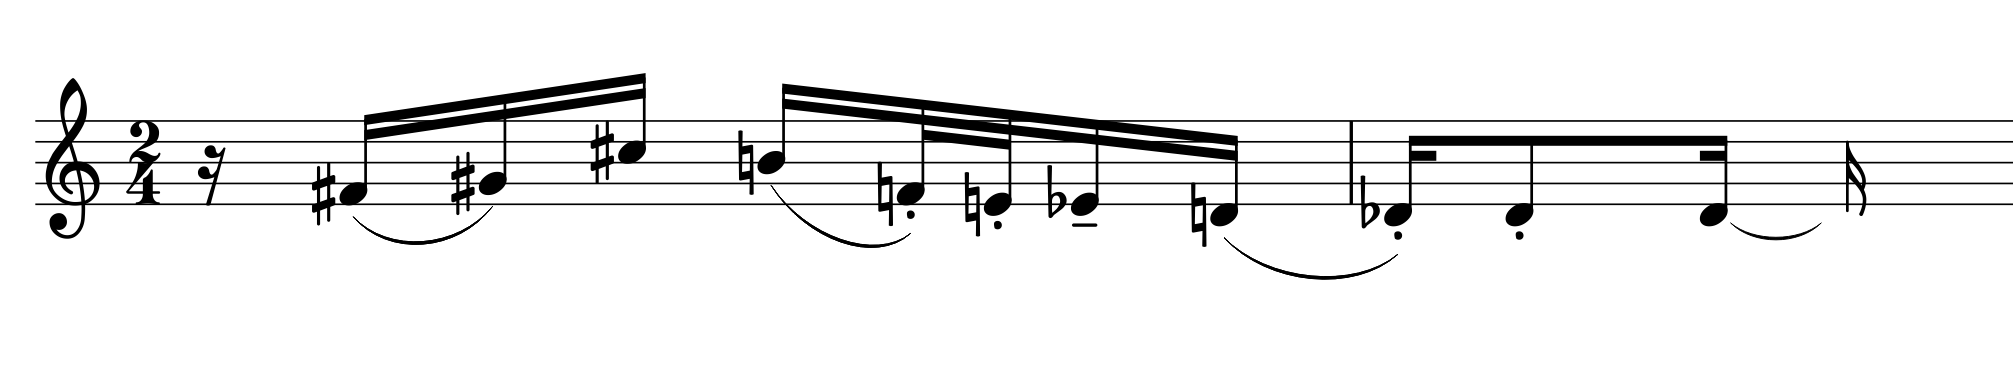
\includegraphics[scale=0.2]{captain}\caption{The Captain}
\label{fig:captain}
\end{figure}


\begin{figure}[H]
\centering
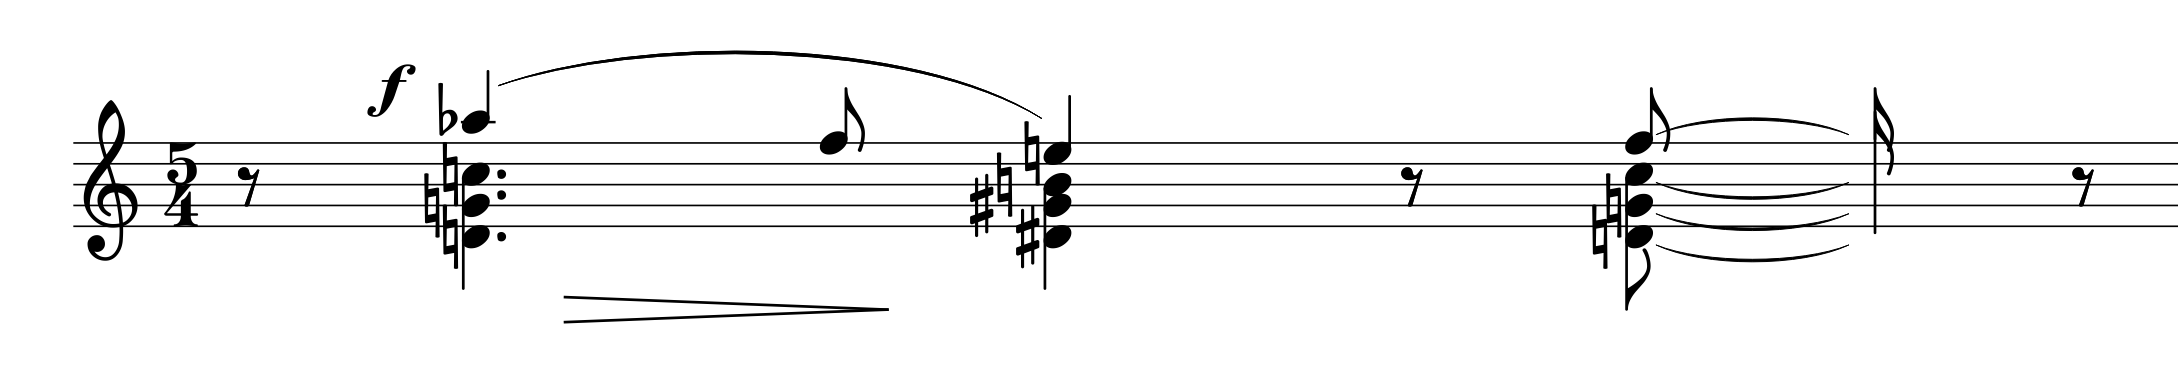
\includegraphics[scale=0.2]{marie}\caption{Marie}
\label{fig:marie}
\end{figure}


\begin{figure}[H]
\centering
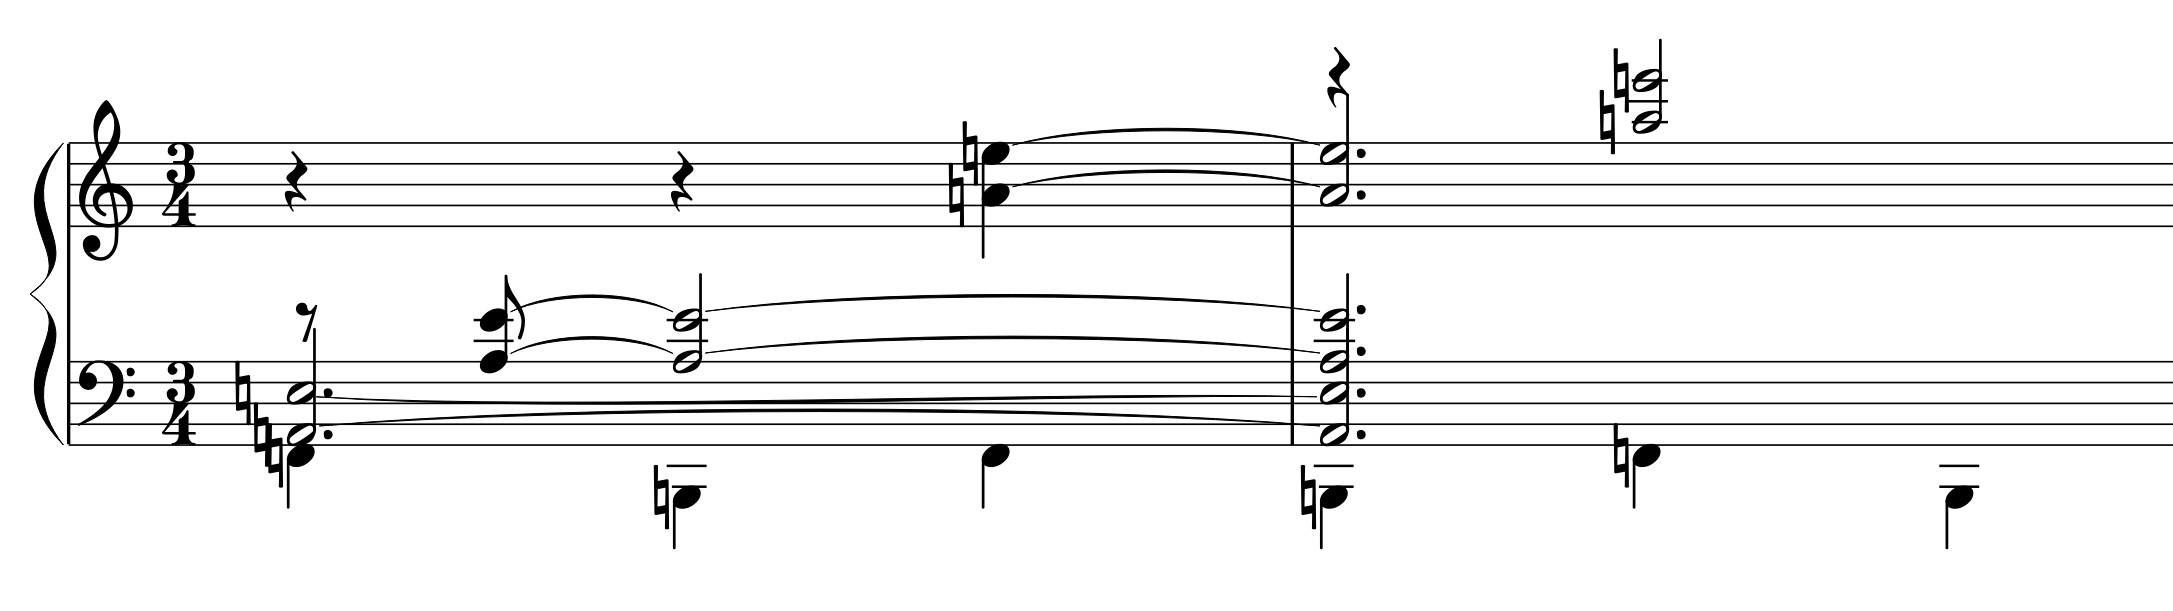
\includegraphics[scale=0.2]{death}\caption{Death}
\label{fig:death}
\end{figure}



\begin{figure}[H]
\centering
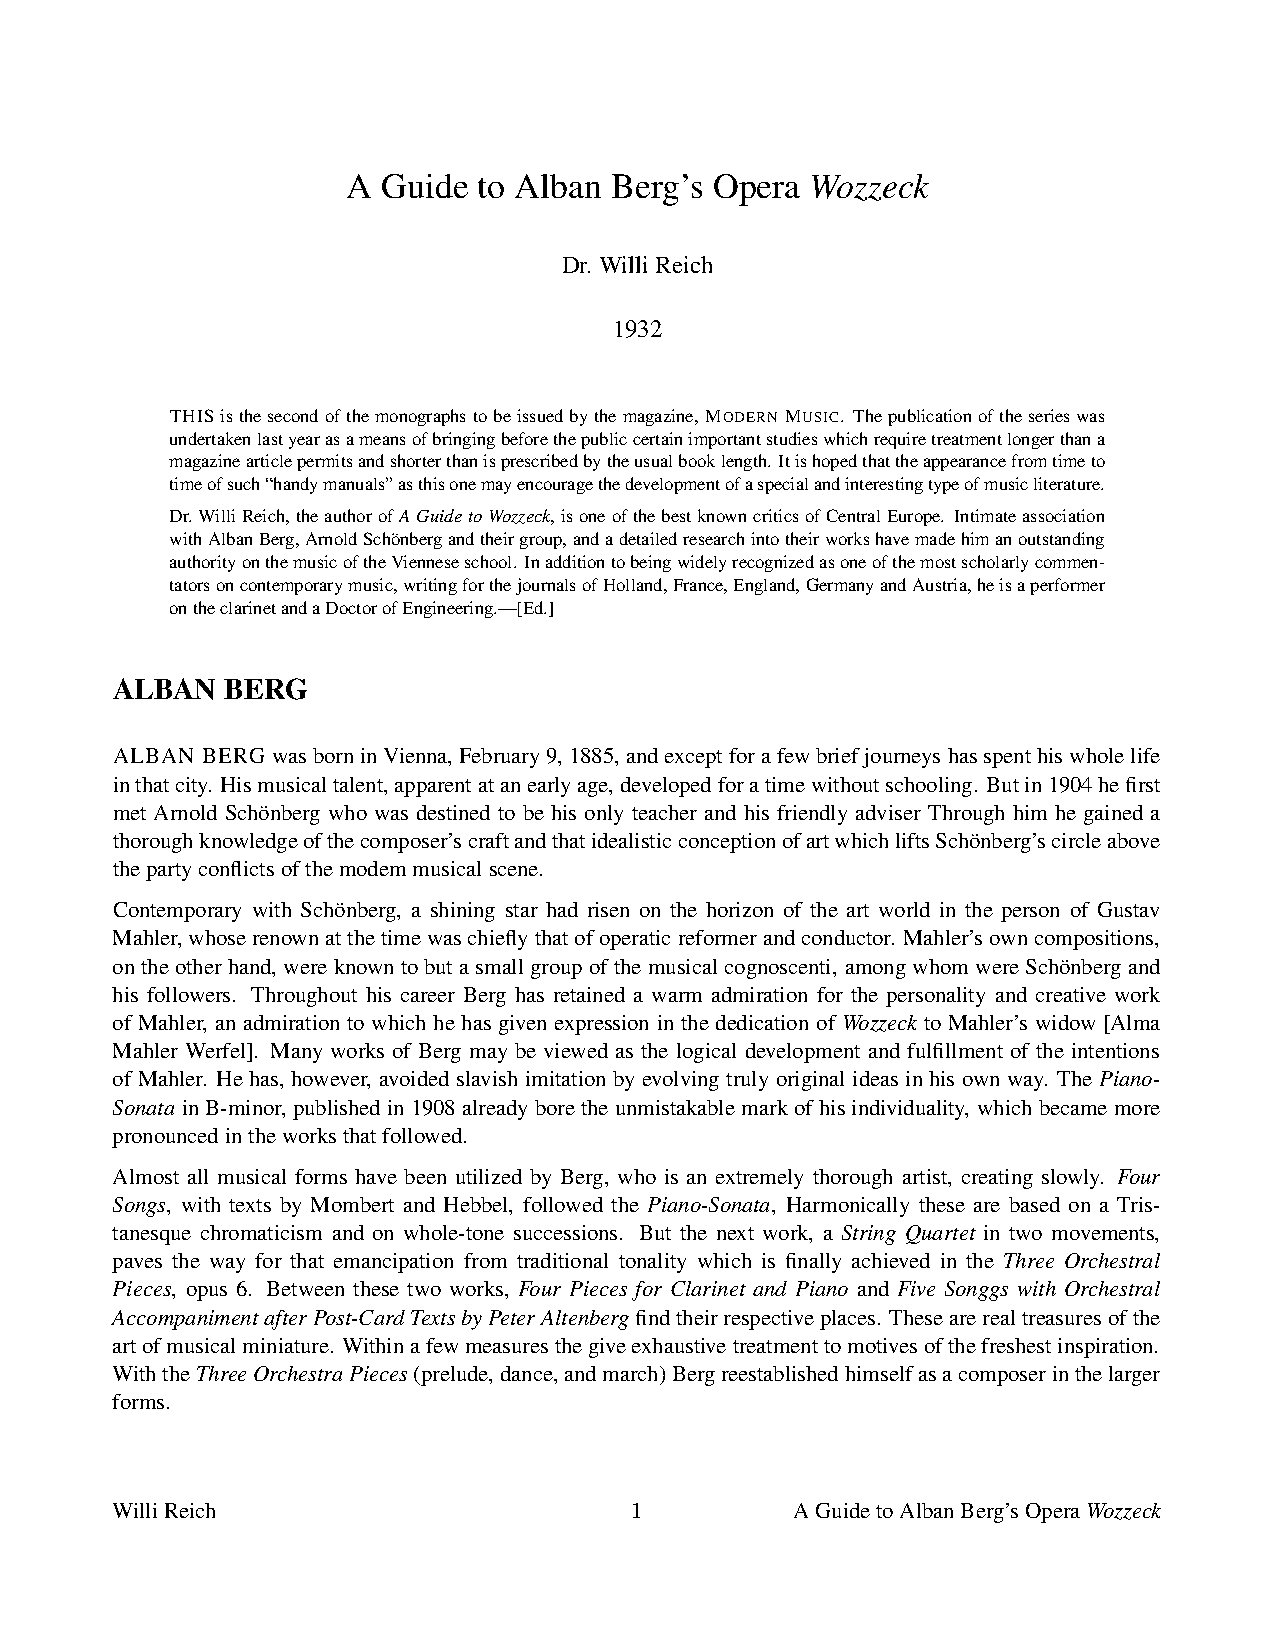
\includegraphics[scale=0.2]{wozzeck}\caption{Wozzeck}
\label{fig:wozzeck}
\end{figure}



\begin{figure}[H]
\centering
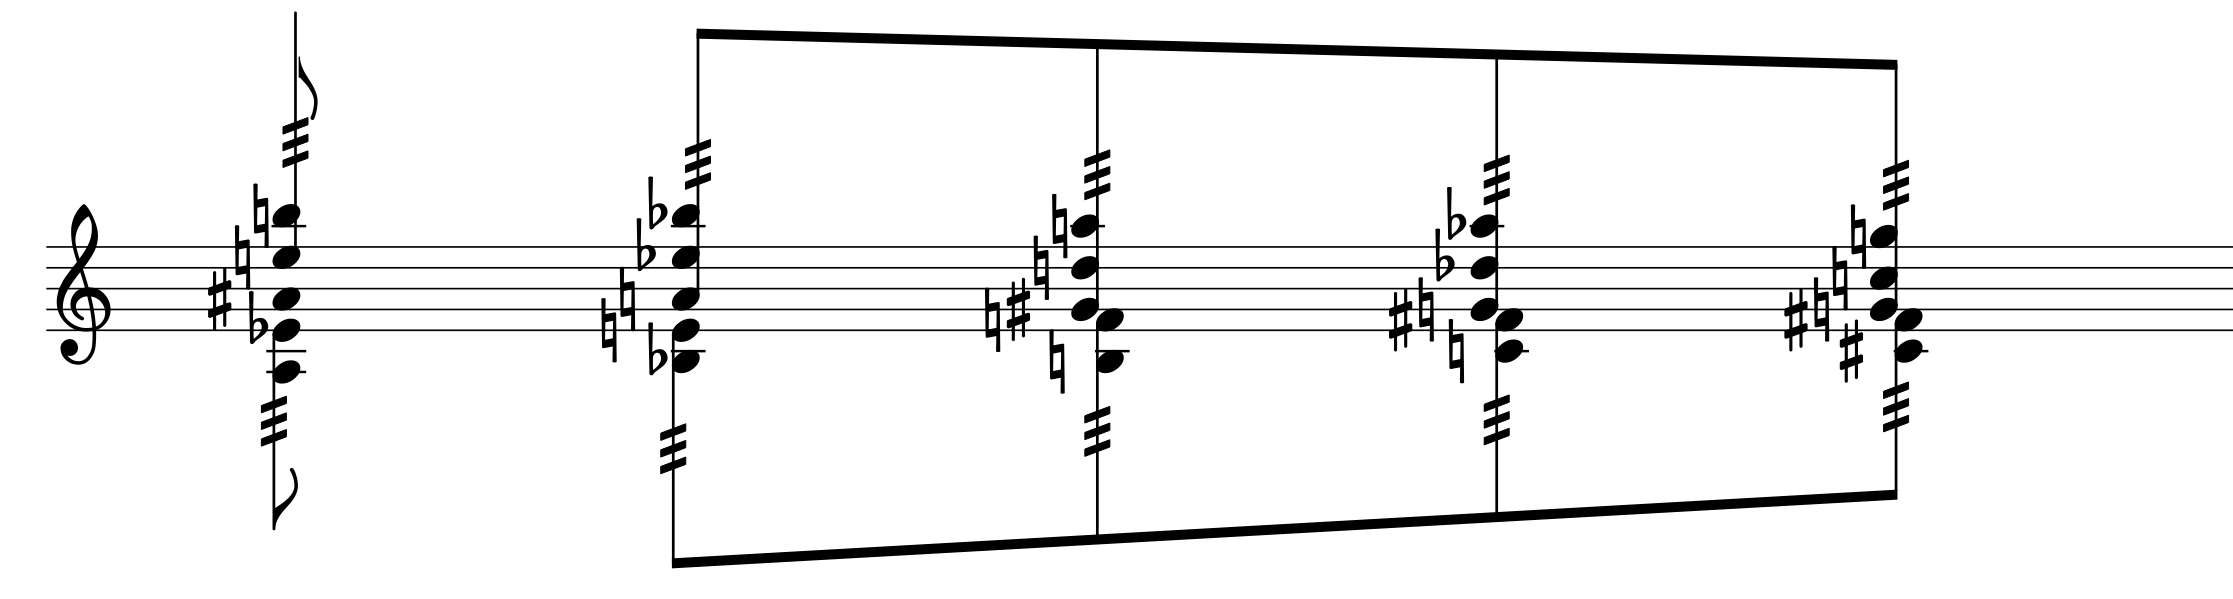
\includegraphics[scale=0.2]{knife}\caption{Knife}
\label{fig:knife}
\end{figure}

Important works after \textit{Wozzeck} include the Chamber concerto, the opera \textit{Lulu} (incomplete at the time of death), after plays by Frank Wedekind and the violin concerto.

The life of the Austrian-German composer in the 30s was terrible. The Nazi regime had basically stated that German music reached its pinnacle with Brahms. Schoenberg went to the United States in 1933, Webern allied himself with Nazis as he needed the work. 

\textit{Lulu} - a monumental work - was abandoned in 1935 as Berg accepted a commission to write the violin concerto. It too had a sad and distressful genesis. The composer died before the first performance (conducted by Webern) with the violinist Krasner (who had commissioned the work) in 1936, in Barcelona.  
 
%%%%%%%%%%%%%%%%%%%%%%%%%%%%%%%%%
\section{Webern: Concerto for nine instruments Op. 24}

\begin{itemize}
\item Listen: \url{https://www.youtube.com/watch?v=vmumBURcHlc}
\item Listen: \url{https://www.youtube.com/watch?v=rIr1xrunnf0}
\item Score: \url{http://imslp.org/wiki/Concerto,_Op.24_%28Webern,_Anton%29}
\end{itemize}

Early studies with Anton Komauer who introduced Webern to Wagner's music but also the songs of Hugo Wolf. Moreover, like Schoenberg, Komauer instilled a thorough grounding in harmony and counterpoint through intense study of Bach. Webern grew up with the music of Strauss and Mahler. Later in his studies, with Professor Guido Adler, Webern got to know the music of Josquin des Pr\`es, Johannes Ockeghem and Heinrich Isaac. Prior to his studies with Schoenberg, Webern had produced little of note, save perhaps for the orchestral work \textit{In Sommerwind}. 

Webern (1883-1945) enrolled in Schoenberg's classes - became friends with Berg - and in four years became a highly skilled composer. Webern was a gifted pianist and cellist and gradually he had to let these skills lapse in favour of composition. Webern's mother died in 1906, (Webern was 23) and this affected him greatly. Even his long-time love and soon to be wife, Wilhelmine M\"ortl realised where her place was in relation to Webern's mother. 

Webern pursued a career as a conductor after finishing his graduate studies which wasn't easy. However he was adequately supported by his father and therefore continued his studies with Schoenberg. In 1908 Webern completed his opus 1, the \textit{Passacaglia} for orchestra. This work is grand in scale and intricate in harmonic detail. It comprises a short theme and 23 variations plus coda. It is also heavily influenced by the death of his mother. As he wrote to Berg, `except for the violin pieces and a few of my orchestra pieces, all of my works from the Passacaglia on relate to the death of my mother...the Passacaglia, the String Quartet, most of the songs, the Second Quartet, the first orchestra pieces, and the second set (with a few exceptions)'. 

Webern studied with Schoenberg until 1908.

Whilst the \textit{Passacaglia} remained tonal (just), the Op.3 and Op.4 sets of songs on poems by Stefan George, begin to see tonality being eschewed for a more expressionistic force. 

Around 1909 when Webern was writing the Op.5 \textit{Five Pieces for string quartet} you can feel the expressionism reacting against any semblance of tonality. These pieces are wrought with tension (but note the heavy use of \textit{sul ponticello}). 

By 1908 Webern was second conductor in the spa town of Bad Ischl - a posting he loathed. Once on the ladder as a conductor (of opera at this time), he remained employed and moved throughout Germany, Austria and the Czech Republic. It is interesting to compare Webern's Op.6 six pieces for large orchestra of 1909 with Schoenberg's 1909 five pieces especially from a point of view of tone colour melody. (Listen to the fourth piece in Webern's set and compare with Schoenberg's \textit{Farben}.) The work is again in memory of his mother and the orchestral forces are used sparingly but aggressively. Remember this is \textbf{before} the \textit{Rite of Spring}.

(Webern's married Wilhelmine around this time and she gave birth to a girl, named `Amalie' after Webern's mother.)

His later set of orchestral works, Op.10 (1911-1913) move even further towards colour harmonies with additional instrumentation. They are scored for four solo strings, seven wind instruments, harmonium, celesta, mandolin, guitar, harp and percussion. Mahler had died in 1911 and some say these works have an `in memoriam' quality too. Movements are short and chiselled. You can hear the serialism wanting to emerge. 

Webern continued to conduct and produce concerts with Schoenberg. Again, the audience was in riotous mood: not the same as the Parisian audience for the \textit{Rite of Spring} as it seemed Schoenberg-school-baiting was now the thing to do. 

The war years for both Webern and Berg were difficult but it seemed Webern, despite his frailties (in particular his eyesight) was keen to do his part. Even after being demobbed at the behest of Zemlinsky, Webern played a role back at home, training young recruits. (As an aside, the relationships between Schoenberg - master- and Berg/Webern pupils are both extensive, convoluted and amusing.)

By around 1920 Werbern had completed the Op.12 songs, the Op.13 set for soprano and orchestra and six songs for for voice and four instruments, Op.14, with words by Georg Trakl. Webern's song style is very expressionist and obviously quite demanding for the soprano. 

By 1920 Webern had ceased to conduct opera and was now living in M\"odling near Vienna. Money remained tight, even when Webern was appointed as modern music adviser for Vienna Radio.  

Schoenberg had invented serialism around 1921. In February 1923, Schoenberg met with some of his pupils and friends to explain his method. Webern was present. Webern's works from Op. 17 \textit{Three Traditional Rhymes for voice and three instruments} (1924) adopt this technique. Interestingly, Webern stuck to traditional compositional techniques as well, using canon (double canon in the Op. 21 Symphony (1927)) and variation form to generate material. 

Schoenberg's Op.23 piano pieces demonstrate the first use of the method. Webern was still relying heavily on the voice to motivate the material. However, in 1927, he ventured back to the strings with his Op.20 trio. 
  
In 1929 Webern conducted in London at the BBC (and during this time, saw his first `talkie'). His quartet for violin, clarinentte, tenor sax and piano was premiered on 13 April 1931. Reviews were, as ever disgusting. Schoenberg visited Vienna in 1933 and this was his last meeting with Webern. Schoenberg was soon to leave Germany. 

Engelbert Dolfuss was elected Chancellor of Austria in 1932 (the year before Hitler was made Chancellor of Germany). Germany then annexed Austria. Webern's conducting career was stopped in its tracks. 

\subsection{Webern Op.24}
 
The \textit{Concerto for nine instruments} (1934) was composed for Schoenberg's 60th birthday. It is one of Webern's most important works. It was premiered at the ISCM festival in Prague on September 4, 1935. Berg died that very same year. Webern conducted the premiere of the violin concerto at the ISCM in Barcelona 19th April, 1936. As Schoenberg wrote to Webern when he returned from Spain:

\begin{quote}
It is too horrible. There goes one of us (who were only a mere three), and now we two must bear this isolation alone. And the saddest aspect is - it had to be the one of us who had success, who at least could have enjoyed that....
\end{quote}


\begin{figure}[H]
\centering
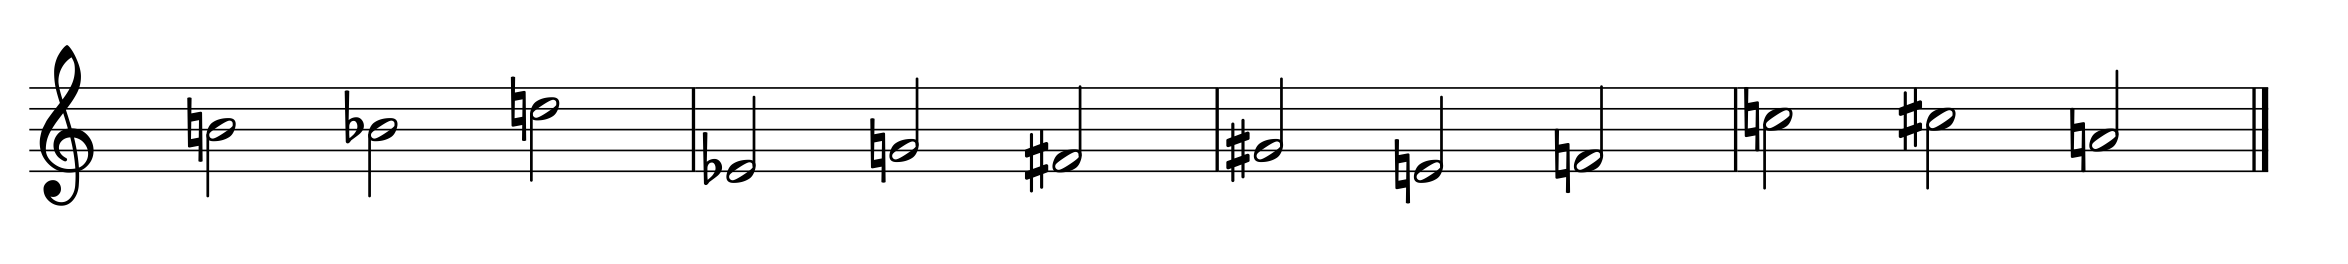
\includegraphics[scale=0.2]{webernop24row}\caption{Webern Op.24 Konzert: Row}
\label{fig:op24row}
\end{figure}

What is so important about this row is that each three note cells is a serial development from the first (RI, R, I).

\begin{figure}[H]
\centering
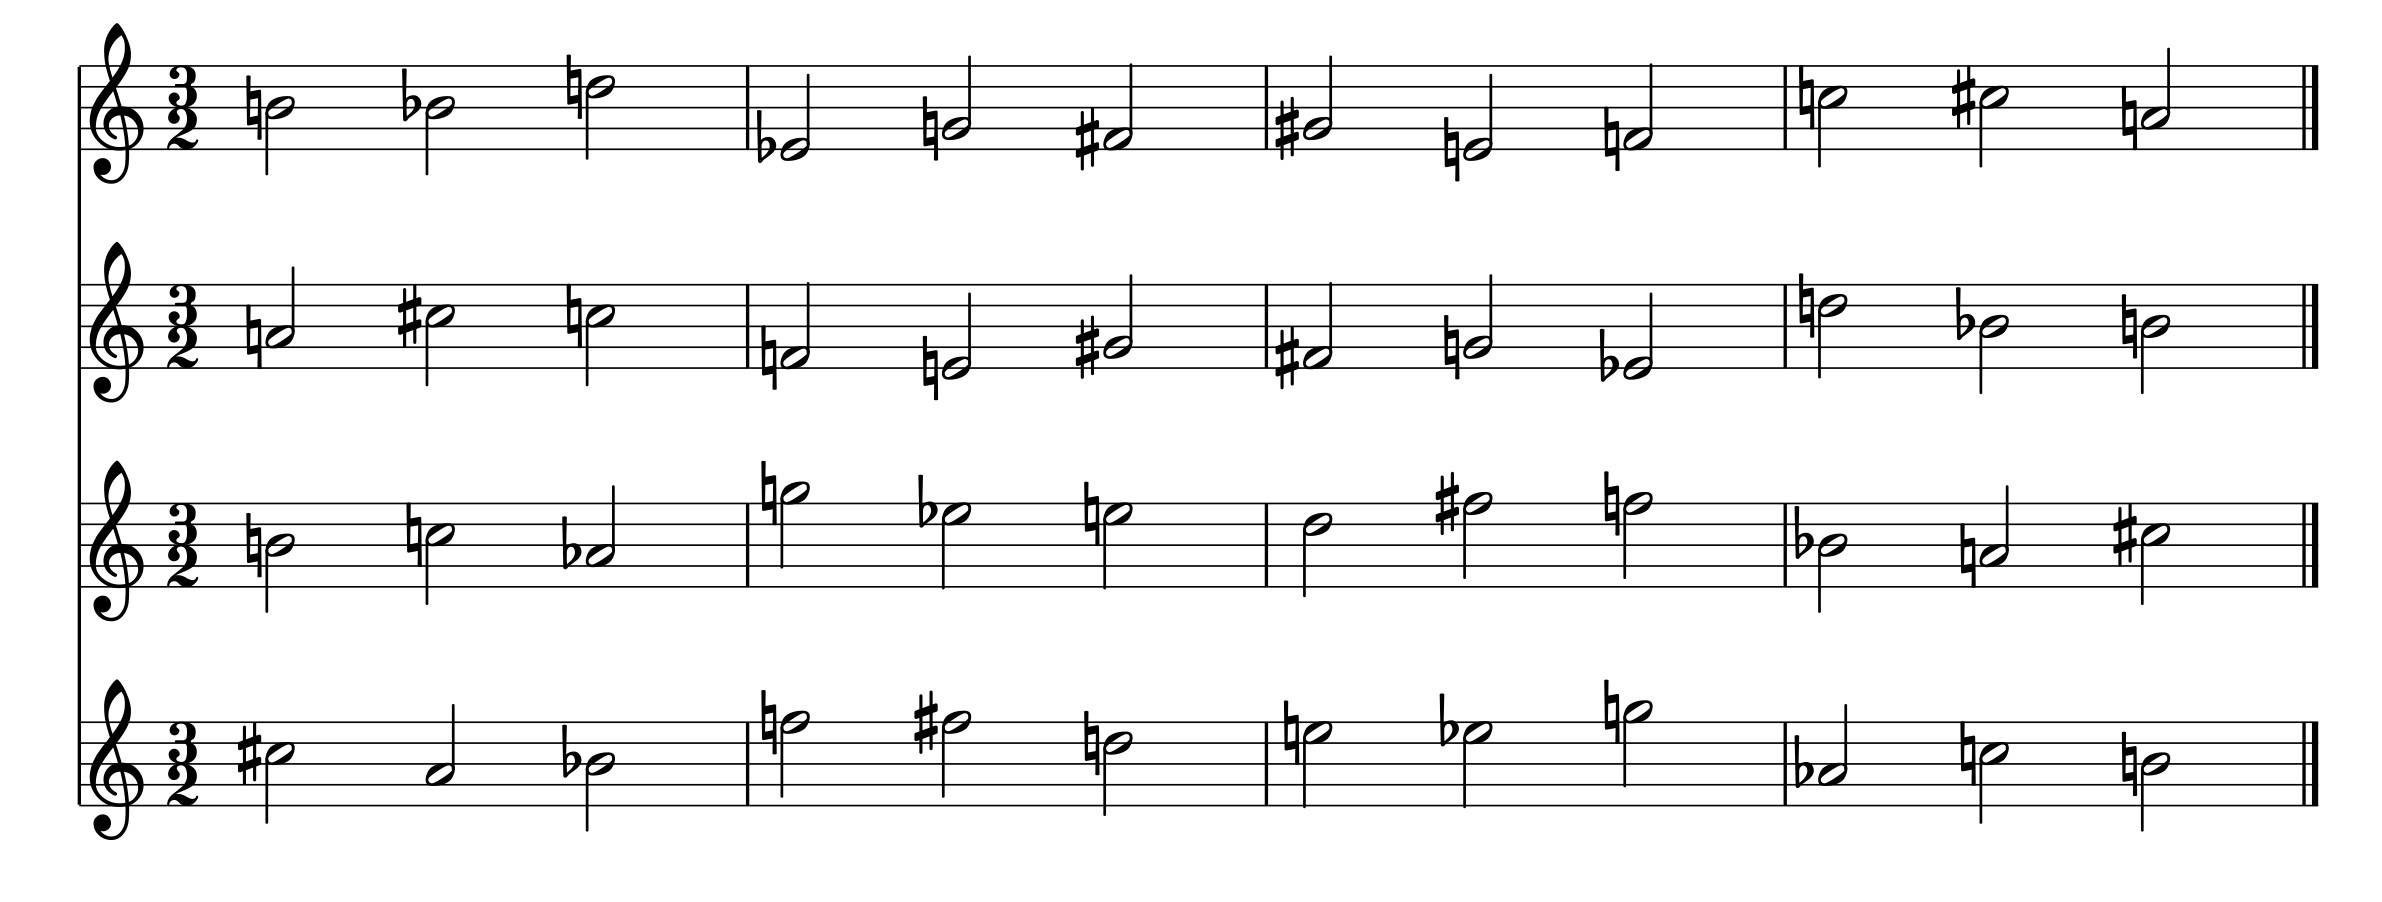
\includegraphics[scale=0.2]{webernrow4-1}\caption{Webern Op.24 Konzert: Row and expansion: Top row is O...what are the rest?}
\label{fig:op24row2}
\end{figure}

This row is given klangfarbenmelodie orchestration and intervallic expansion (minor 2nds becoming minor 9ths). It is clear that the rows are split between piano and the other instruments or shared between the two. The next entrance is piano:

\begin{figure}[H]
\centering
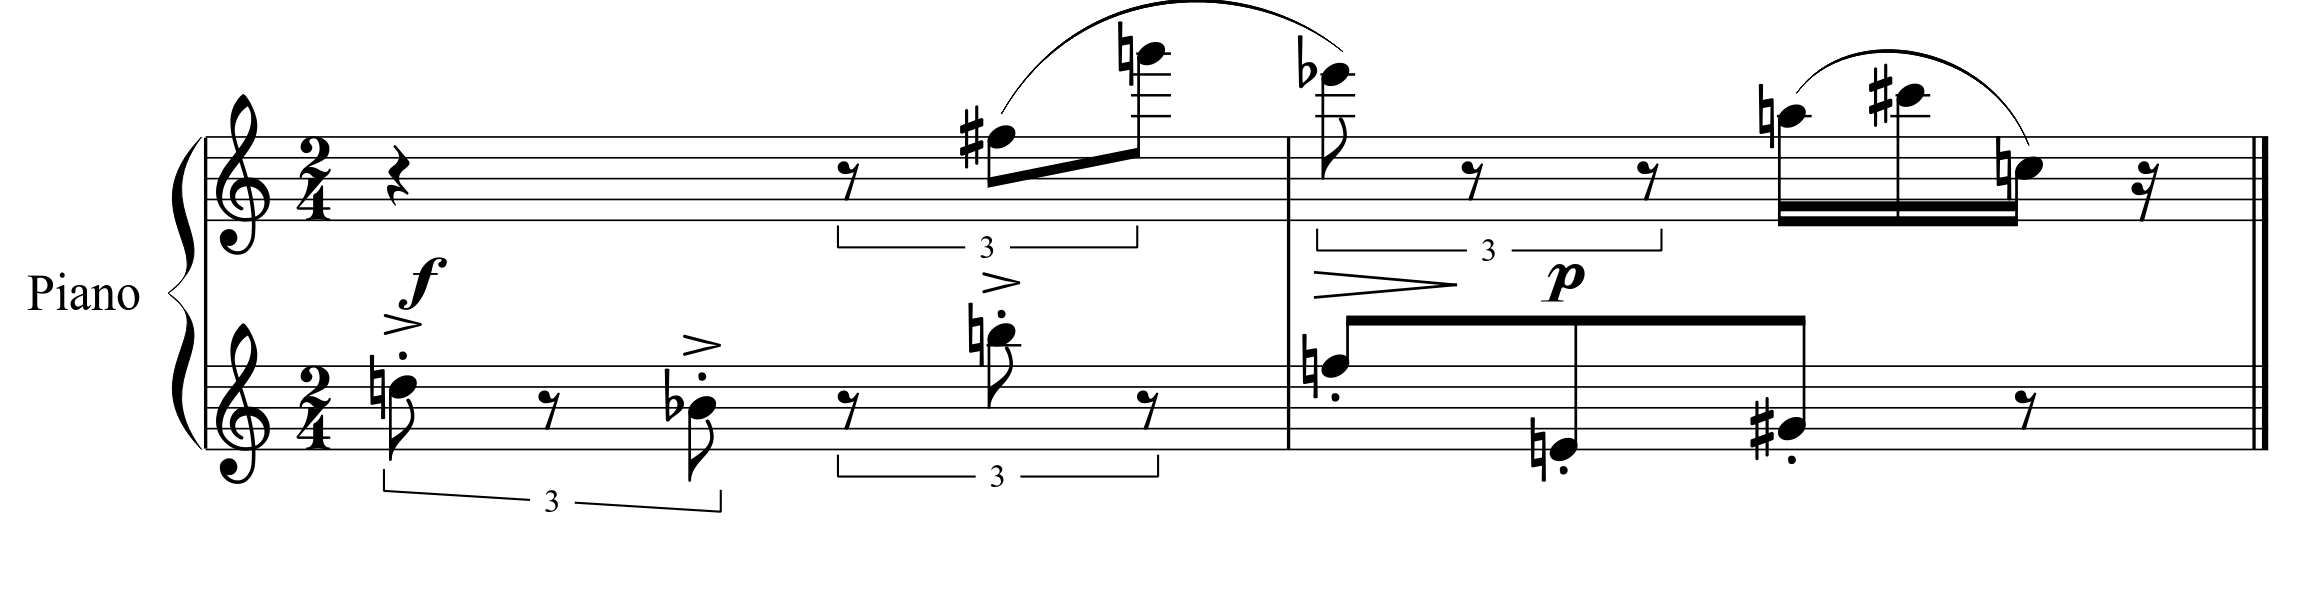
\includegraphics[scale=0.2]{webernop24row2-1}\caption{Webern Op.24 Konzert: Piano entry}
\label{fig:op24row}
\end{figure}




Webern also demonstrated his musical talent through unique orchestrations and arrangements of works by others. In particular Bach's \textit{Ricercata} from the \textit{Musical Offering} (1935). Here the instrumentation changes constantly. 

Towards the end of the 1930s Webern was living a relatively quiet life with his wife (his children had left home). Financially he was not doing well, earning but a little from private teaching. As many composers had done in the past, his Op.28 

\subsection{Final works}
Key works after the Konzert:
\begin{itemize}
\item ``Das Augenlicht'' for choir and orchestra, Op.26 (1935)
\item Variations for Piano Op.27 (1936)
\item String quartet Op.28 (1937-1938) using BACH
\item Cantata Op.29 (1938-1939)
\item Variations for Orchestra Op. 30 (1940)
\item Cantata Op.31 (1941-1943)
\end{itemize}

The Nazis invaded annexed Austria on March 12th, 1938. The defeat of the German army at Stalingrad in February 1943 marked a turning point in the war. Webern's son Peter was conscripted. Webern celebrated his 60th birthday in Vienna on 3rd December 1943. Even Webern was called up again to `air-raid protection police'.  

As the war was drawing to its horrific close and the Russian army was approaching Vienna, Webern and his wife moved to Mittersill, some 60 km south of Salzburg for three weeks. Vienna fell on/around 13th April. Hitler committed suicide on April 30th 1945. The Third Reich surrendered on 8th May. Webern, after recovering from serious illness found out he was to be offered both a teaching position and a permanent conducting post seemed set fair. On September 15th Webern was shot by an American undercover soldier by mistake (see \citep[p216]{hayes1995anton}). 

Webern's legacy as a leaner, meaner serialist (more so than Schoenberg and Berg) endeared him to the new avant-garde of Boulez and Stockhausen. 


\bibliographystyle{apalike} 
\bibliography{../../usss_coursebook/ajmbib}
%\printglossary

\backmatter
%\printindex

\end{document}
